%% Computers & Geosciences submission package generated from the TU_Lag manuscript.
%% Official C&G checklist: single-column double-spaced manuscript,
%% author-date references, code availability, and separate cover letter/highlights files.
\documentclass[a4paper,fleqn]{cas-sc}

\usepackage[authoryear]{natbib}
\usepackage{amsmath,amssymb}
\usepackage{booktabs,array}
\usepackage{longtable}
\usepackage{placeins}
\usepackage{siunitx}
\usepackage{url}
\usepackage{lineno}
\usepackage{graphicx}
\usepackage{float}
\usepackage{setspace}

\setlength{\emergencystretch}{2em}

\begin{document}
\let\WriteBookmarks\relax
\def\floatpagepagefraction{1}
\def\textpagefraction{.001}
\shorttitle{Aquifer-test transformation uncertainty}
\shortauthors{Lin}

\title [mode = title]{A reproducible benchmark for transformation uncertainty in aquifer-test parameter inference}

\author[1]{Ying-Fan Lin}
\ead{yflin1110@cycu.edu.tw}
\credit{Conceptualization, methodology, software, validation, formal analysis, investigation, data curation, visualization, writing--original draft, writing--review and editing, funding acquisition.}

\address[1]{Department of Civil Engineering, Chung Yuan Christian University, Taoyuan, Taiwan}

\begin{abstract}
Aquifer-test transmissivity and storage are not direct observations; they are inferred by fitting a response model to drawdown. This paper presents a reproducible computational benchmark for quantifying how that drawdown-to-parameter transformation affects inferred aquifer properties before they enter groundwater models, pumping-capacity calculations, or response-time estimates. Four analytical interpretations--Theis confined flow, Hantush--Jacob leakage, lagging Darcy without leakage, and lagging Darcy with leakage--are fitted to controlled numerical responses and two field pumping tests. A 10,000 scenario groundwater-flow ensemble generated 160,012 fitted interpretation records across homogeneous, leaky, finite-boundary, heterogeneous, and combined settings. The benchmark provides support-matched reference parameters, analytical limiting checks, grid sensitivity checks, and scenario-conditioned model factors. Analytical verification confirmed physical consistency in 22 of 25 limiting cases, and numerical responses aligned with analytical references in 30 of 32 configurations. Benchmark-transfer regressions predicted the 90th percentile absolute log model factor with cross-validated $R^2$ values of 0.48, 0.51, and 0.55 for transmissivity, storage, and response time. Application to the Massachusetts fractured-bedrock and Lovelock Valley basin-fill cases produced benchmark-conditioned model-factor COV values of 0.61--0.90 and 0.31--0.51, respectively. Model-averaged decision diagnostics showed that the selected interpretation can understate hydraulic capacity and response-time spread. The workflow treats lagging Darcy as one candidate interpretation, not a universal replacement, and reports transformation uncertainty through response residuals, benchmark support, field applicability, and inherited decision consequences.
\end{abstract}

\begin{keywords}
Aquifer testing \sep Computational hydrogeology \sep Uncertainty quantification \sep Numerical benchmark \sep Model-form error \sep Reproducible workflow
\end{keywords}

\maketitle
\printcredits
\doublespacing
\linenumbers

\section{Introduction}

Groundwater studies and water resource decisions often depend on aquifer test parameters. Groundwater supply assessment, capture analysis, dewatering design, contaminant migration evaluation, geothermal screening, and regional groundwater models commonly use transmissivity and storage estimates as site evidence \citep{freeze_cherry1979,bear1979,anderson2015}. Most site reports derive these parameters by fitting analytical solutions, including classical confined flow, leakage, delayed yield, wellbore storage, and generalized radial flow interpretations, to observed drawdown records \citep{theis1935,cooper_jacob1946,hantush_jacob1955,boulton1954,papadopulos_cooper1967,neuman1975,barker1988}. Advanced hydraulic tomography and geostatistical inversion can then map hydraulic properties across a site or aquifer system \citep{kitanidis1995,yeh_liu2000,liu_illman2007,illman2009}.

Drawdown is measured directly; transmissivity and storage are inferred through an interpretation model. Stochastic hydrogeology and inverse modeling provide mature tools for propagating parameter uncertainty through flow calculations and site-scale predictions \citep{dagan1989,gelhar1993,rubin2003,yeh1986,carrera_neuman1986,beven_binley1992,hill_tiedeman2007,doherty2015}. Groundwater uncertainty research also addresses model structure, conceptual models, hydrostratigraphy, boundary conditions, management forecasts, data worth, and multimodel prediction \citep{refsgaard2006,rojas2008,poeter_anderson2005,ye2010,tsai2010,gupta2012,tsai_elshall2013,xu_valocchi2015,guillaume2016,fienen2025}. Those methods operate after a groundwater model or model ensemble has been defined. Aquifer test interpretation occurs upstream, where model-form error can enter transmissivity and storage before those values become spatial model inputs, prior distributions, or engineering design parameters. This upstream step matches the broader role of transformation models, which trace derived properties back to the measurements and transformations that produced them \citep{phoon_kulhawy1999a,phoon_kulhawy1999b}.

The upstream interpretation step separates the present work from related uncertainty problems. Slug-test support studies treat test estimates as weighted spatial averages over a near-well support volume \citep{beckie_harvey2002}. Pumping-test upscaling studies ask how interpreted transmissivity and storativity values should inform regional groundwater model parameters and prior distributions \citep{manewell2022,manewell2024}. Aquifer-scale inference studies define when pumping tests can recover effective transmissivity and storage in heterogeneous aquifers \citep{naderi_gupta2023}. Groundwater BMA and conceptual model studies combine predictions after a model ensemble and parameter estimation strategy has been specified \citep{li_tsai2009,tsai2010,tsai_elshall2013}. The analysis here targets the earlier conversion from a drawdown record to apparent transmissivity, storage, leakage, and response-time parameters.

Groundwater decisions often depend on hydraulic capacity or response time rather than on the fit of a single drawdown curve. Pumping tests are used to size construction dewatering and groundwater control systems. Required pumping capacity scales with transmissivity, and the response time of pressure propagation scales with storage divided by transmissivity \citep{powers2007}. Groundwater model averaging and management studies show that a single best model can underestimate prediction uncertainty when model structure or parameter estimation methods remain uncertain \citep{li_tsai2009,tsai2010,tsai_elshall2013}. Aquifer test transformation uncertainty can therefore enter management analysis as under-reported spread in transmissivity, storage, or hydraulic diffusivity.

Reported parameter variability can reflect both subsurface heterogeneity and the interpretation process used to estimate parameters. If a classical instantaneous response model omits temporal response structure, such as exchange between fractures and matrix, weakly connected pores, delayed drainage, or lagged storage release \citep{warren_root1963,lin_yeh2017,lin_huang_yeh2019}, fitting can redistribute the mismatch into transmissivity, storage, leakage, or response-time parameters. The resulting parameter spread can then resemble spatial variability \citep{sanchez_vila1999,manewell2022}. Groundwater interpretation therefore needs fitted parameters to be reported with log model factor diagnostics, model complexity checks, identifiability diagnostics, boundary and leakage alternatives, and validation evidence.

The present work develops a reproducible, benchmark-conditioned workflow for aquifer-test transformation uncertainty. Four analytical transformations--Theis confined, Hantush--Jacob leaky, lagging Darcy without leakage, and lagging Darcy with leakage--separate classical confined flow, conventional leakage, temporal memory, and combined leakage and memory behavior. Their role is to provide a controlled set of drawdown-to-parameter mappings for estimating how model-form choice changes apparent transmissivity, storage, leakage, and response-time quantities.

The evidence chain links response-scale residuals, controlled numerical reference values, reproducible field diagnostics, and groundwater decision quantities. A 10,000 scenario numerical groundwater-flow benchmark provides known reference parameters, analytical limiting behavior, numerical consistency tests, observation-layout variation, and screened model factor distributions. Benchmark-transfer regressions relate the response diagnostics to model-factor magnitude and place the Massachusetts fractured bedrock and Lovelock Valley basin fill field tests on the same conditional uncertainty scale \citep{cho2004pumping,cho2008characterization,nadler2020report,nadler2020data}. The fitted interpretations are then propagated into model-averaged hydraulic capacity and response-time indices, distinguishing response fitting from the quantities inherited by later groundwater calculations.
\section{Methods}

\subsection{Transformation uncertainty associated with interpretation models}

The generic transformation model has the following form \citep{phoon_kulhawy1999b}:

    \begin{equation}
    \xi_d = \mathcal{T}(\xi_m,\epsilon),
    \label{eq:phoon_transform}
    \end{equation}

\noindent where $\xi_d$ is the derived or design property, $\xi_m$ is the measured property, $\mathcal{T}(\cdot)$ is the generic transformation function, and $\epsilon$ is transformation uncertainty. Equation~\ref{eq:measured_components} defines the measured property ($\xi_m$) by integrating a trend ($t$), inherent variability ($w$), and measurement error ($e$):

    \begin{equation}
    \xi_m = t+w+e.
    \label{eq:measured_components}
    \end{equation}

\noindent A first order second moment approximation expresses the variance of the derived property as contributions from inherent variability, measurement error, and transformation uncertainty:

    \begin{equation}
    \operatorname{Var}(\xi_d) \approx
    \left(\frac{\partial \mathcal{T}}{\partial w}\right)^2\operatorname{Var}(w)
    +
    \left(\frac{\partial \mathcal{T}}{\partial e}\right)^2\operatorname{Var}(e)
    +
    \left(\frac{\partial \mathcal{T}}{\partial \epsilon}\right)^2\operatorname{Var}(\epsilon).
    \label{eq:second_moment}
    \end{equation}

\noindent Equations~\ref{eq:phoon_transform},~\ref{eq:measured_components}, and~\ref{eq:second_moment} define the uncertainty vocabulary used here. The two field cases provide response and parameter evidence for an interpretation diagnostic, while complete measurement error budgets and independent heterogeneity measurements remain separate evidence needs. The diagnostic therefore separates field response residuals, apparent parameter spread, model form support, identifiability, support scale, and decision inheritance. A full source-by-source uncertainty matrix is provided in Supplementary Table~S1.

\subsection{Pumping test interpretation model as a transformation model}

The measured pumping test vector for observation well $i$ is:

    \begin{equation}
    \mathbf{y}_{m,i}=\{s_i(t_j), Q, r_i, b, t_j\}_{j=1}^{n_i},
    \label{eq:measurement_vector}
    \end{equation}

\noindent where $s_i(t_j)$ is observed drawdown, $Q$ is pumping rate, $r_i$ is radial distance from the pumping well, $b$ is aquifer thickness, and $t_j$ is elapsed time. The interpretation model $M$ transforms this measured response into an inferred parameter vector:

    \begin{equation}
    \boldsymbol{\theta}_{M,i}=\mathcal{T}_M(\mathbf{y}_{m,i},\epsilon_{M,i}).
    \label{eq:aquifer_transform}
    \end{equation}

The classical Darcy interpretation yields:

    \begin{equation}
    \boldsymbol{\theta}_{D,i}=(S_{D,i},T_{D,i}),
    \label{eq:darcy_parameters}
    \end{equation}

\noindent whereas the lagging Darcy interpretation yields:

    \begin{equation}
    \boldsymbol{\theta}_{L0,i}=(S_{L0,i},T_{L0,i},\tau_{q,i},\tau_{s,i}).
    \label{eq:lagging_parameters}
    \end{equation}

\noindent The subscript $L0$ denotes the lagging Darcy interpretation without leakage. The lagging leaky interpretation adds a leakage factor:

    \begin{equation}
    \boldsymbol{\theta}_{LL,i}=(S_{LL,i},T_{LL,i},B_{LL,i},\tau_{q,i},\tau_{s,i}),
    \label{eq:lagging_leaky_parameters}
    \end{equation}

\noindent with Equation~\ref{eq:lagging_parameters} recovered as the diagnostic limit $B_{LL}\rightarrow\infty$. This distinction is important because the original lagging model for a leaky confined aquifer combines aquitard leakage with lagged storage and flow responses \citep{lin_yeh2017}. The present field analysis implements both lagging interpretations and treats $B_{LL}$, $\tau_q$, and $\tau_s$ as fitted response parameters specific to the interpretation model; independent field constraints would be needed to convert them into site specific physical quantities.

\noindent Equations~\ref{eq:measurement_vector},~\ref{eq:aquifer_transform},~\ref{eq:darcy_parameters},~\ref{eq:lagging_parameters}, and~\ref{eq:lagging_leaky_parameters} make the conversion from drawdown to parameters explicit. The measured quantity is $s_i(t)$, whereas the transformation $\mathcal{T}_M$ generates $S$, $T$, and any additional response parameters. Unresolved timing structure can remain as a transformation residual if the interpretation model lacks a temporal response component required by the observed response.

The fitting process can then compress that residual structure into $S$ and $T$, producing parameter compensation and inflating interpreted spatial variability across observation wells. The lagging parameters represent temporal memory effects rather than absorbing them entirely into apparent $S$ and $T$. Here, $\tau_q$ is a lumped flux-gradient memory or relaxation time, and $\tau_s$ is a lumped storage-release response lag. Both serve as diagnostic response times within the transformation model. The central hydrogeologic question is how much of the classical drawdown mismatch and interpreted $S$-$T$ variability aligns with unresolved temporal dynamics after the analysis includes classical leakage and boundary alternatives.

The transformation model is indexed by interpretation choice. Let $a$ denote an interpretation model, such as a Theis, leaky, delayed yield, wellbore storage, generalized radial flow, dual porosity, numerical inverse, or lagging interpretation. The apparent parameter produced by interpretation model $a$ is written as

    \begin{equation}
    \boldsymbol{\theta}_{a,i}^{\mathrm{app}} =
    \mathcal{H}_{a}\left(\boldsymbol{\theta}^{\ast},\mathbf{g}_{i},\mathbf{q},\mathbf{b},\mathbf{w}_{i}\right)
    + \boldsymbol{\delta}_{a}(\boldsymbol{\Pi}_{i})+\mathbf{e}_{a,i},
    \label{eq:pathway_indexed}
    \end{equation}

\noindent where $\boldsymbol{\theta}^{\ast}$ is the support scale aquifer property that would be needed for an independent reference test, $\mathbf{g}_{i}$ is well geometry, $\mathbf{q}$ is the pumping schedule, $\mathbf{b}$ denotes boundary and support assumptions, $\mathbf{w}_{i}$ is the observation window, $\boldsymbol{\delta}_{a}$ is the transformation bias specific to interpretation model $a$ and conditioned on dimensionless controls $\boldsymbol{\Pi}_{i}$, and $\mathbf{e}_{a,i}$ is residual error associated with the interpretation model. Because the present field cases lack independent observations of $\boldsymbol{\theta}^{\ast}$, Equation~\ref{eq:pathway_indexed} provides diagnostic traceability from measured drawdown to fitted parameters.

\subsection{Field data sets and pumping test operations}

\subsubsection{Massachusetts fractured bedrock pumping test}

The Massachusetts field case comes from a fractured crystalline bedrock site in eastern Massachusetts, United States \citep{cho2004pumping,cho2008characterization}. The 24 hour pumping test occurred in an open bedrock borehole with a 15 cm diameter and a 30 m depth, featuring one major water bearing fracture within the upper 23 m. The small bedrock well network samples drawdown responses controlled by fracture connectivity and radial distance from the pumping borehole.

The retained Massachusetts subset comprises 12 observation wells and 420 drawdown observations. Observation well files record elapsed time and drawdown, while a coordinate table defines the local well layout and distances from the pumping well. Although the original test included variable pumping rate stages (approximately 4, 7, 0, and 2 L/min), this diagnostic treats the retained drawdown records as a constant rate response with $Q=\SI{1.2e-4}{m^3.s^{-1}}$ to match current analysis inputs. This approach standardizes the transformation comparison across wells and defines the Massachusetts case as a diagnostic of the retained constant rate subset. The variable rate stages remain documented as an applicability condition for the retained subset, and the data manifest records the copied raw inputs and their source folder.

\subsubsection{Lovelock Valley basin fill pumping/recovery test}

The Lovelock Valley field case is multiwell pumping test 2. The analysis treats it as an independent basin fill field case separate from the Massachusetts fractured bedrock data. Lovelock Valley is a basin fill valley in the lower Humboldt River Basin of Nevada. The U.S. Geological Survey report describes a valley floor groundwater system bounded and underlain by consolidated rock with low permeability and filled by older and younger alluvial deposits \citep{nadler2020report}. The younger basin fill contains the main water bearing deposits: colluvium from the surrounding mountains, fluvial sediments associated with the Humboldt River, and lacustrine clays and silts deposited by Lake Lahontan. The report distinguishes coarser alluvium, fluvial deposits, and Lahontan clays and silts as hydrogeologic units evaluated with slug tests, multiwell pumping tests, and groundwater modeling \citep{nadler2020report}. This setting contrasts with the Massachusetts fractured bedrock case because observation wells may respond through layered basin fill aquifers and leaky shallow fine grained units.

The associated public data release provides the pumping schedule, well distances, processed drawdown/recovery strings, and PEST observation weights \citep{nadler2020data}. Pumping Well 10, an agricultural well completed in the coarser alluvium, discharged at approximately \SI{0.381}{m^3.s^{-1}} from 28 November 2017 10:53 to 4 December 2017 11:28. The retained observation wells span 0.6--9.6 miles from the pumping well and include responses from both coarse alluvial wells and shallow Lahontan clay/silt observation wells.

The Lovelock processing follows the structure of the public data release. The response is simulated by superimposing a pumping rate step and a shutoff step so that recovery observations contribute to the fit. The log response offset in Equation~\ref{eq:eta} is set to 0.05 ft (\SI{0.0152}{m}) to match the report's threshold for drawdown detection. The analysis uses the drawdown/recovery observations, excludes the pumping well, excludes observation strings with zero weight, and retains observation wells whose maximum corrected drawdown exceeds the report's detection threshold. This leaves seven observation wells and 520 processed observations. Lovelock is analyzed as a separate field case because it differs in site scale, preprocessing, observation weighting, and environmental correction. The retained spatial support for both field cases is reported at the start of the field diagnostic results in Figure~\ref{fig:layout}.

\subsection{Analytical interpretation models and fitting protocol}

The interpretation protocol applies each field case's observation records, pumping representation, and well coordinates to four main analytical interpretations. Theis confined provides the classical reference without leakage, Hantush--Jacob provides the conventional leaky aquifer reference, lagging Darcy without leakage tests temporal memory without leakage, and lagging Darcy with leakage tests combined leakage and memory behavior. This analytical response framing follows aquifer test literature that interprets drawdown through response solutions for confined, leaky, delayed yield, wellbore storage, or generalized radial flow conditions \citep{theis1935,cooper_jacob1946,hantush_jacob1955,boulton1954,papadopulos_cooper1967,neuman1975,barker1988}. Auxiliary late time regression is used as a screening diagnostic outside the field comparison based on the full observation record. The lagging responses are evaluated in the Laplace domain, and the Stehfest algorithm \citep{stehfest1970} inverts them to the time domain.

For the formal lagging leaky interpretation, the finite radius kernel in the Laplace domain is

    \begin{equation}
    \alpha_{LL}^{2}(p)=
    \left(\frac{pS}{T}+\frac{1}{B^2}\right)
    \frac{1+p\tau_q}{1+p\tau_s},
    \label{eq:lagging_leaky_kernel}
    \end{equation}

\noindent where $p$ is the Laplace variable, $\alpha_{LL}$ is the lagging leaky radial decay term, and $S$, $T$, $B$, $\tau_q$, and $\tau_s$ are the fitted storage, transmissivity, leakage, flux lag, and storage lag parameters for the interpretation model. The corresponding constant rate response for a finite radius well is written as

    \begin{equation}
    \bar{s}_{LL}(p)=
    \frac{Q K_0(\alpha_{LL}r)}
    {\pi r_w^2 p^2 K_0(\alpha_{LL}r_w)+2\pi r_w T p\alpha_{LL}K_1(\alpha_{LL}r_w)}.
    \label{eq:lagging_leaky_laplace}
    \end{equation}

\noindent where $\bar{s}_{LL}(p)$ is drawdown in Laplace space, $r_w$ is pumping well radius, $r$ is observation distance, and $K_0(\cdot)$ and $K_1(\cdot)$ are modified Bessel functions of the second kind. Equations~\ref{eq:lagging_leaky_kernel} and~\ref{eq:lagging_leaky_laplace} recover the lagging Darcy interpretation without leakage as $B\rightarrow\infty$ and recover the leaky interpretation without lag for a finite radius well as $\tau_q=\tau_s=0$. Numerical checks confirmed these limiting cases before field fitting.

For both field cases, nonlinear least squares with multiple starts independently estimates fitted parameters for each observation well in log parameter space, applying the log model factor in response (Equation~\ref{eq:eta}) as the data term. The final refit uses a weak maximum a posteriori (MAP) objective, appending lognormal prior residuals to the data residuals to avoid hard boundary solutions in weakly identifiable directions. The prior centers are $S=10^{-3}$, $T=5\times10^{-5}\,\mathrm{m^2\,s^{-1}}$, and $\tau_q=\tau_s=10^3$ s. The standard deviations of the log scale priors are 3.0 and 2.0 for classical $S$ and $T$, and 2.0, 1.8, 3.0, and 3.0 for lagging $S$, $T$, $\tau_q$, and $\tau_s$. Broad fitting bounds remain $S\in[10^{-8},1]$, $T\in[10^{-8},10^{-1}]$, and lag times in $[10^{-4},10^{9}]$ seconds for the lagging refit without leakage. The lagging leaky field fit uses the same log response data term, $B\in[1,10^6]$ m, and lag time bounds of $[10^{-4},10^{7}]$ seconds, with flags reported when $B$ or a lag direction approaches a bound. Local MAP tradeoff diagnostics are computed from the numerical Jacobian of the final log response MAP residual vector at each fitted optimum.

The Hantush--Jacob leaky interpretation fits $S$, $T$, and leakage factor $B$ using

    \begin{equation}
    s_H(t)=\frac{Q}{4\pi T}W\left(u,\frac{r}{B}\right), \qquad
    u=\frac{r^2S}{4Tt},
    \label{eq:hantush_field}
    \end{equation}

\noindent where $s_H(t)$ is Hantush--Jacob drawdown, $W(u,r/B)$ is the leaky aquifer well function, and $u$ is the dimensionless time variable. A first type boundary diagnostic is also retained outside the four main analytical interpretations to avoid attributing drawdown controlled by boundaries to lagging response alone. This sensitivity check uses an effective recharge image well:

    \begin{equation}
    s_{CH}(t)=\frac{Q}{4\pi T}\left[E_1\left(\frac{r^2S}{4Tt}\right)
    -E_1\left(\frac{r_I^2S}{4Tt}\right)\right],
    \label{eq:constant_head_image}
    \end{equation}

\noindent where $s_{CH}(t)$ is the constant head image well drawdown diagnostic, $E_1(\cdot)$ is the exponential integral, and $r_I$ is an effective image well distance used to represent boundary sensitivity. This auxiliary fit tests whether late time flattening could be explained by an equivalent boundary response outside the four full record interpretation models.
\subsection{Transformation model factor in the response}

At the scale of the measured response, model factors describe transformation uncertainty when an indirect model converts observations into design parameters \citep{phoon_kulhawy1999a,phoon_kulhawy1999b}. Pumping tests require this idea to retain time and well indices because early, middle, and late time responses can carry different model errors. Unresolved temporal dynamics--such as lagged flux or delayed storage release--should appear as structured drawdown model factors before inverse algorithms interpret the mismatch as spatial differences in aquifer properties.

For observation well $i$ at time $t_j$, the observed and modeled log responses are

    \begin{equation}
    z_{\mathrm{obs},i,j}=\log\left[s_{\mathrm{obs},i}(t_j)+c\right],
    \qquad
    z_{M,i,j}=\log\left[s_{M,i}(t_j;\boldsymbol{\theta}_{M,i})+c\right],
    \label{eq:log_response}
    \end{equation}

\noindent where $s_{\mathrm{obs},i}$ is observed drawdown, $s_{M,i}$ is drawdown predicted by interpretation model $M$, $\boldsymbol{\theta}_{M,i}$ is the fitted parameter vector for well $i$, and $c$ is a case specific positive offset that prevents unstable logarithms near zero drawdown. The Massachusetts analysis uses $c=\SI{0.001}{m}$, and the Lovelock analysis uses $c=0.05$ ft (\SI{0.0152}{m}) following the report's detection threshold. The time and well indexed log model factor is

    \begin{equation}
    \eta_{M,i,j}=z_{\mathrm{obs},i,j}-z_{M,i,j}
    =\ln \left(\frac{s_{\mathrm{obs},i}(t_j)+c}{s_{M,i}(t_j;\boldsymbol{\theta}_{M,i})+c}\right),
    \label{eq:eta}
    \end{equation}

\noindent with the corresponding multiplicative model factor

    \begin{equation}
    F_{M,i,j}=\exp(\eta_{M,i,j}).
    \label{eq:model_factor}
    \end{equation}

\noindent A value of $F_{M,i,j}=1$ indicates that the interpretation model reproduces the observed response at that time and well after fitting. Values above or below 1 indicate observation-model ratios on the drawdown scale. The dispersion of the log model factor for any diagnostic group $G$ is

    \begin{equation}
    SD_{\epsilon,M}(G)=
    \sqrt{\frac{1}{|G|-1}\sum_{(i,j)\in G}
    \left(\eta_{M,i,j}-\bar{\eta}_{M,G}\right)^2},
    \label{eq:sd_epsilon}
    \end{equation}

\noindent where $G$ may be the full response record, a single well, a field case, or an early, middle, or late time window; $|G|$ is the number of observations in that group; and $\bar{\eta}_{M,G}$ is the group mean log model factor. This definition makes the reported $SD_{\epsilon}$ an interpretation dependent and group dependent log model factor dispersion. When a conventional coefficient of variation for the multiplicative model factor is desired, the lognormal relation is

    \begin{equation}
    COV_{F,M}(G)=\sqrt{\exp\left[SD_{\epsilon,M}(G)^2\right]-1}.
    \label{eq:cov_model_factor}
    \end{equation}

\noindent The response variance ratio is

    \begin{equation}
    VR_{\epsilon}(G)=\frac{\operatorname{Var}_{(i,j)\in G}(\eta_{L,i,j})}
    {\operatorname{Var}_{(i,j)\in G}(\eta_{D,i,j})}.
    \label{eq:vr_eta}
    \end{equation}

Equations~\ref{eq:log_response}--\ref{eq:vr_eta} define the response-level transformation diagnostics. The analysis reports $SD_{\epsilon,M}(G)$ because the log factor is symmetric for overprediction and underprediction and remains stable near small drawdown after adding $c$. Each well is split into early, middle, and late time windows using time quantiles within each well to diagnose whether the lagging Darcy model primarily reduces timing related model factor dispersion.

\subsection{Variability in inferred hydraulic properties and trend adjustment}

To diagnose parameter compensation, all positive fitted parameters are evaluated on the log scale, consistent with common hydrogeologic treatment of strongly positive and spatially variable hydraulic properties \citep{dagan1989,gelhar1993,rubin2003}. The lognormal coefficient of variation is

    \begin{equation}
    COV_X=\sqrt{\exp(\sigma_{\ln X}^{2})-1},
    \label{eq:cov}
    \end{equation}

\noindent where $X$ denotes a positive fitted parameter and $\sigma_{\ln X}^{2}$ is the variance of $\ln X$ across wells. Variability in inferred parameters is compared using

    \begin{equation}
    VR_X=\frac{\operatorname{Var}_i(\ln X_{L,i})}{\operatorname{Var}_i(\ln X_{D,i})}, \quad X\in\{S,T\}.
    \label{eq:vr_parameter}
    \end{equation}

\noindent Equations~\ref{eq:cov} and~\ref{eq:vr_parameter} quantify raw variability in inferred hydraulic properties. Interpreting that variability as geologic heterogeneity requires external site evidence in addition to the fitted parameter spread.

Raw variance across wells can mix hydrogeologic heterogeneity, observation geometry, and parameter compensation introduced by the model. Variability in inferred hydraulic properties after trend adjustment is evaluated using two simple regressions:

    \begin{equation}
    \ln X_{M,i}=\beta_{0,M}+\beta_{r,M}\ln r_i+u_{M,i},
    \label{eq:distance_trend}
    \end{equation}

\noindent and

    \begin{equation}
    \ln X_{M,i}=\beta_{0,M}+\beta_{x,M}x_i+\beta_{y,M}y_i+u_{M,i}.
    \label{eq:xy_trend}
    \end{equation}

\noindent where $\beta_{0,M}$ is the intercept, $\beta_{r,M}$ is the coefficient for log distance, $\beta_{x,M}$ and $\beta_{y,M}$ are coordinate coefficients, $x_i$ and $y_i$ are well coordinates, and $u_{M,i}$ is the trend residual. The variance of $u_{M,i}$ is reported as detrended variability in inferred hydraulic properties. Equations~\ref{eq:distance_trend} and~\ref{eq:xy_trend} function as diagnostic trend adjustments; a geostatistical representation would require additional spatial support.

\subsection{Model complexity, tradeoff, and validation}

The candidate interpretation models include different numbers of fitted parameters, so residual improvement is evaluated alongside model complexity diagnostics. Approximate AIC and BIC are computed as

    \begin{equation}
    AIC_M=n\ln \left(\frac{RSS_M}{n}\right)+2k_M,
    \label{eq:aic}
    \end{equation}

\noindent and

    \begin{equation}
    BIC_M=n\ln \left(\frac{RSS_M}{n}\right)+k_M\ln n,
    \label{eq:bic}
    \end{equation}

\noindent where $n$ is the number of response observations, $RSS_M$ is the residual sum of squares for model $M$, and $k_M$ is 2 for Theis confined, 3 for Hantush--Jacob leaky, 4 for lagging Darcy without leakage, and 5 for lagging Darcy with leakage \citep{akaike1974,schwarz1978}. Equations~\ref{eq:aic} and~\ref{eq:bic} provide support for the response model after complexity adjustment, complementing multiple model and predictive uncertainty practices in groundwater studies \citep{poeter_anderson2005,ye2010,doherty2015}. Local MAP covariance matrices are used to compute selected correlations among $\ln T_L$, $\ln S_L$, $\ln \tau_q$, and $\ln \tau_s$, addressing the general calibration need to identify parameter tradeoffs, compensation, and lack of uniqueness \citep{yeh1986,hill_tiedeman2007,xu_valocchi2015}.

The validation diagnostic excludes one observation well at a time to test spatial transfer. The validation diagnostic predicts log parameters for each excluded well from the remaining 11 wells using the log distance trend in Equation~\ref{eq:distance_trend}, and then simulates the excluded well using these predicted parameters. This test follows the predictive logic of cross validation \citep{vehtari2017} and focuses on spatial transfer across the retained observation network. It directly tests whether patterns in fitted parameters across wells generalize beyond the specific wells used to define them.

\subsection{Numerical groundwater-flow benchmark and analytical verification}

Independent values of the true support scale transmissivity, storage, leakage factor, and response time parameters are unavailable in field pumping tests. The main controlled check therefore uses a prescribed numerical groundwater-flow generator before the two field cases are interpreted. MODFLOW 6 is used here as a reproducible groundwater-flow solver \citep{langevin2017,bakker2016}, while the method itself applies to any simulator that can generate comparable transient drawdown fields. The numerical simulations supply transient responses from Darcy groundwater-flow equations, and the four analytical interpretations then convert those responses into apparent aquifer parameters. This design tests the front-end transformation from drawdown to parameters under controlled numerical aquifer conditions.

The numerical ensemble comprises 10,000 fully simulated pumping-test scenarios in ten classes: homogeneous confined flow, distributed vertical leakage, finite no-flow boundary, constant head boundary, heterogeneous hydraulic conductivity, anisotropic heterogeneous hydraulic conductivity, heterogeneous storage, heterogeneous leakage, heterogeneous boundary, and combined leakage and boundary settings (Figure~\ref{fig:mf6design}). Each class contributes 1000 scenarios. The design spans grid spacings of 5.0--10.0 m, square domains of 405--1205 m, six observation layouts with 3--5 wells between near well and far field support, transient records with 20--40 logarithmically spaced output times over 1--10 days, and water level noise levels of 0--0.01 m. Heterogeneous cases use correlated lognormal hydraulic conductivity or storage fields, with anisotropy included as a separate class. Each numerical response is then refitted by the four analytical interpretations, generating 160,012 fitted interpretation and well records.

The reference parameter is defined before fitting. Homogeneous, leaky, and boundary scenarios with uniform properties use the assigned confined transmissivity and storage values. Heterogeneous scenarios use a scenario-specific effective pumping support rather than a fixed radial average. The effective support radius is computed from hydraulic diffusivity, pumping duration, maximum observation distance, leakage length where present, and boundary or domain limits. Hydraulic conductivity and storage are then averaged with diffusion-decay weights clipped by that effective support, with arithmetic, annular, and fixed-radius sensitivity summaries retained as secondary comparisons. In the 10,000 scenario benchmark, the median effective support radius is \SI{139}{m}, with a 10th--90th percentile range of \SI{99}{m}--\SI{298}{m}. This definition is reported explicitly because a numerical cell value is not the same object as a pumping-test parameter.

The numerical design defines the benchmark scope through two controlled checks. Closed-form limiting comparisons verify that the implemented analytical models reduce to their expected reference solutions: Hantush--Jacob to Theis as the leakage factor becomes large, lagging Darcy to Theis when response lags collapse, lagging leaky Darcy to lagging Darcy when leakage becomes inactive, and lagging leaky Darcy to Hantush--Jacob when the lag times are equal. Numerical consistency comparisons then relate homogeneous confined simulations to Theis and distributed leakage simulations to Hantush--Jacob across grid spacings of 2.5--20 m. Model factors are summarized for fitted records without active parameter boundary flags and with $\Delta BIC \leq 10$ relative to the best interpretation for the same response. Field use is further screened by applicability criteria that classify each field case as conservative, sensitivity, lower complexity, or non-primary relative to the numerical scenario classes.

\begin{figure}
\centering
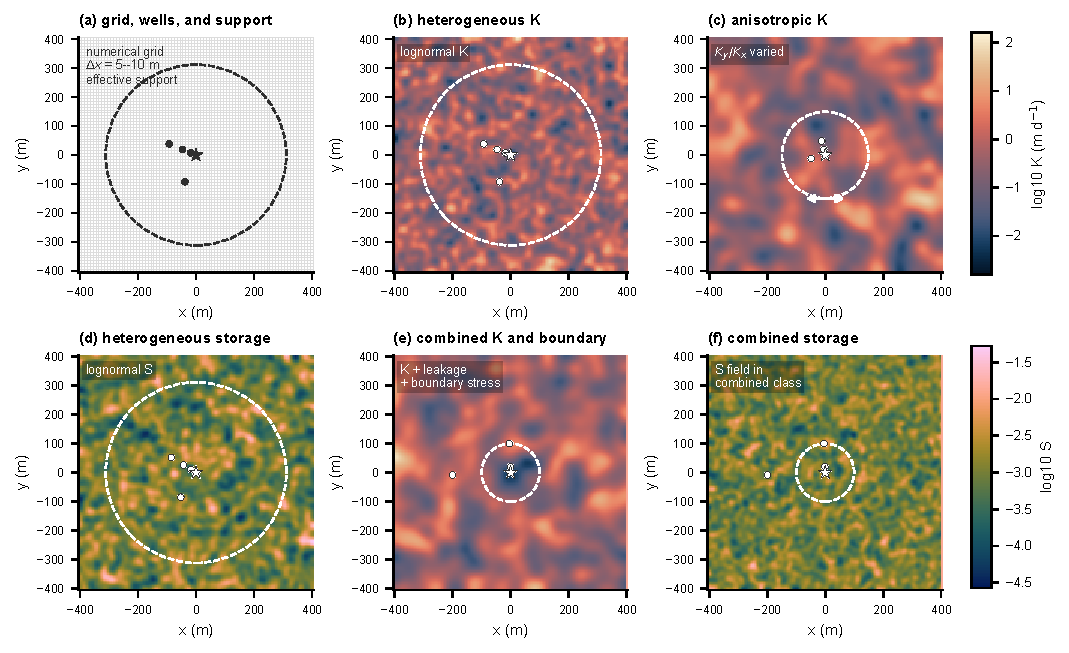
\includegraphics[width=\linewidth]{fig13_mf6_benchmark_design.pdf}
\caption{Numerical groundwater-flow benchmark design with MODFLOW 6 through (a) the finite-difference grid, extraction well, observation wells, and scenario-specific effective support envelope for the aquifer-test reference; (b) a representative heterogeneous hydraulic conductivity field; (c) a representative anisotropic hydraulic conductivity field; (d) a representative heterogeneous storage field; (e) combined leakage, boundary, hydraulic conductivity, and storage conditions for transformation stress; and (f) paired numerical response classes for the four analytical interpretations. The numerical fields define controlled drawdown responses for interpretation by the four analytical solutions.}
\label{fig:mf6design}
\end{figure}

For each numerical drawdown record, the four analytical interpretations are fitted independently. The response level model factor remains the log factor in Equation~\ref{eq:eta}. The benchmark also defines parameter transformation model factors

    \begin{equation}
    M_{T,M}=\frac{T_{\mathrm{app},M}}{T_{\mathrm{ref}}},
    \qquad
    M_{S,M}=\frac{S_{\mathrm{app},M}}{S_{\mathrm{ref}}},
    \label{eq:mf6_parameter_factor}
    \end{equation}

\noindent where $T_{\mathrm{app},M}$ and $S_{\mathrm{app},M}$ are apparent parameters obtained by interpretation model $M$, and $T_{\mathrm{ref}}$ and $S_{\mathrm{ref}}$ are the support matched numerical reference values. The reported model factor coefficient of variation is computed from the standard deviation of the log model factor:

    \begin{equation}
    COV_M=\left[\exp\left(\sigma_{\ln M}^2\right)-1\right]^{1/2}.
    \label{eq:mf6_cov}
    \end{equation}

\noindent Equation~\ref{eq:mf6_cov} is used separately for transmissivity, storage, hydraulic control capacity, and response time. The resulting values are scenario-conditioned transformation priors applied to field cases when the field diagnostics resemble the benchmark class.

The closed-form analytical comparisons are retained as supplementary controlled checks. They confirm that the implemented analytical solutions and fitting routines recover clean Theis and leaky responses under prescribed generating models. The 10,000 scenario numerical benchmark is the main controlled basis for estimating conditional transformation model factors for field interpretation.

\subsection{Benchmark transfer to field diagnostics}

The numerical benchmark provides known reference values, whereas the field cases provide response and interpretation diagnostics. A benchmark-transfer analysis estimates the scale of model-factor uncertainty that a field pumping test may inherit when its diagnostics resemble portions of the benchmark. The predictor set is restricted to diagnostics that can be computed for both numerical and field tests. For benchmark scenario $k$, the response-diagnostic vector is

    \begin{equation}
    \mathbf{z}_{k} =
    \left[
    SD_{\epsilon,M},
    p_{\mathrm{BIC},M},
    h_{M},
    g_{M,M'}
    \right]_{M,M'\in\mathcal{M}},
    \label{eq:transfer_features}
    \end{equation}

\noindent where $SD_{\epsilon,M}$ is the pathway-specific log model factor dispersion, $p_{\mathrm{BIC},M}$ is the fraction of observation wells for which model $M$ has the lowest BIC, $h_M$ is the boundary-hit fraction for fitted parameters, and $g_{M,M'}$ is the fractional reduction in $SD_{\epsilon}$ between two interpretation models. These quantities describe the diagnostic behavior of the fitted response.

For each numerical scenario, the transferred quantity is the 90th percentile absolute log model factor for transmissivity, storage, or response time:

    \begin{equation}
    y_{q,k}=Q_{0.90}\left(\left|\ln M_{q,M,i}\right|\right),
    \qquad q\in\{T,S,t_c\}.
    \label{eq:transfer_target}
    \end{equation}

\noindent A nonlinear regression ensemble $f_q(\mathbf{z}_k)$ is estimated separately for each $q$ using one row per numerical scenario. Five-fold validation keeps all wells and interpretation records from a numerical scenario in the same fold. The fitted relation is then evaluated at the field diagnostic vector $\mathbf{z}_{\mathrm{field}}$ to obtain a benchmark-conditioned estimate $\widehat{y}_{q,\mathrm{field}}$. For reporting on a familiar coefficient-of-variation scale, the 90th percentile absolute log factor is converted to a lognormal-equivalent COV by

    \begin{equation}
    COV^{(90)}_{q,\mathrm{field}}
    =
    \left[
    \exp\left\{
    \left(\frac{\widehat{y}_{q,\mathrm{field}}}{1.645}\right)^2
    \right\}-1
    \right]^{1/2}.
    \label{eq:transfer_cov90}
    \end{equation}

\noindent Equation~\ref{eq:transfer_cov90} defines a benchmark-conditioned sensitivity bracket at the represented response-diagnostic scale. The regression estimates model-factor magnitude for field diagnostics while the numerical responses and the four analytical interpretations retain separate roles.

\subsection{Model-averaged management diagnostic}

The management diagnostic tests whether a later groundwater control or management calculation can inherit an overconfident aquifer test input if interpretation uncertainty is collapsed into one fitted parameter set. The calculation follows the Bayesian model averaging logic used in groundwater uncertainty studies, where predictions are combined with posterior model probabilities and uncertainty is separated into components associated with candidate models and parameter estimation methods \citep{hoeting1999,li_tsai2009,tsai_elshall2013}. The model set comprises the four fitted aquifer test interpretations in the present analysis. Their fitted $T$ and $S$ values are propagated into two analytical decision quantities: hydraulic control capacity, which is proportional to $T$, and characteristic response time, which is proportional to $S/T$.

For field case or well group $i$, the posterior weight of interpretation model $M$ is approximated from the BIC values:

    \begin{equation}
    w_{M,i}=
    \frac{
    \exp \left[-0.5\left(BIC_{M,i}-BIC_{\min,i}\right)\right]
    }
    {
    \sum_{M'\in\mathcal{M}}
    \exp \left[-0.5\left(BIC_{M',i}-BIC_{\min,i}\right)\right]
    },
    \label{eq:bma_weight}
    \end{equation}

\noindent where $\mathcal{M}$ contains Theis confined flow, Hantush--Jacob leakage, lagging Darcy without leakage, and lagging Darcy with leakage. Equal prior model probabilities are used so that the weights reflect complexity-adjusted support from the field response data.

Because strict BIC weights can collapse onto one best model, the diagnostic also uses a variance window weight. This weighting follows the model window treatment of Li and Tsai \citep{li_tsai2009}, who showed that fixed narrow model windows can overrate best models and underestimate multimodel uncertainty:

    \begin{equation}
    w^{V}_{M,i}=
    \frac{
    \exp \left[-0.5\Delta BIC_{M,i}/s_{\Delta BIC,i}\right]
    }
    {
    \sum_{M'\in\mathcal{M}}
    \exp \left[-0.5\Delta BIC_{M',i}/s_{\Delta BIC,i}\right]
    },
    \label{eq:bma_variance_window_weight}
    \end{equation}

\noindent where $\Delta BIC_{M,i}=BIC_{M,i}-BIC_{\min,i}$ and $s_{\Delta BIC,i}$ is the sample standard deviation of the four $\Delta BIC$ values for well or field group $i$, with a lower bound of 1. This variance window diagnostic serves as a sensitivity check that retains plausible analytical interpretations when the information criterion spread itself is large.

For either strict BIC weights or variance window weights, a model-derived decision variable $x_{M,i}$ is averaged as a discrete BMA distribution:

    \begin{equation}
    p(x_i\mid D)=
    \sum_{M\in\mathcal{M}}
    w^{(\cdot)}_{M,i}
    \delta\left(x_i-x_{M,i}\right),
    \label{eq:bma_decision_distribution}
    \end{equation}

\noindent where $w^{(\cdot)}_{M,i}$ denotes either Equation~\ref{eq:bma_weight} or Equation~\ref{eq:bma_variance_window_weight}. The two decision variables are hydraulic diffusivity and characteristic response time:

    \begin{equation}
    D_{M,i}=\frac{T_{M,i}}{S_{M,i}},
    \qquad
    t_{c,M,i}=\frac{r_i^2S_{M,i}}{4T_{M,i}},
    \label{eq:management_diffusivity_time}
    \end{equation}

\noindent where $D_{M,i}$ is hydraulic diffusivity, $t_{c,M,i}$ is the Theis characteristic response time for observation distance $r_i$, and $T_{M,i}$ and $S_{M,i}$ are the transmissivity and storage inferred by interpretation model $M$. These analytical decision indices screen the uncertainty inherited by later, project specific groundwater management calculations.

For a hydraulic control or dewatering capacity calculation, the required capacity scales with transmissivity. If the calculation is based on the selected interpretation $M_i^*=\arg\max_M w^{V}_{M,i}$, the robust capacity factor is

    \begin{equation}
    R^{C}_{i}=
    \max \left[
    1,
    \frac{Q_{0.95}\{T_i\mid D\}}{T_{M_i^*,i}}
    \right],
    \label{eq:robust_capacity_factor}
    \end{equation}

\noindent and the capacity shortfall probability relative to the selected interpretation is

    \begin{equation}
    P^{C}_{i}=\Pr(T_i>T_{M_i^*,i}\mid D).
    \label{eq:capacity_violation}
    \end{equation}

\noindent For monitoring and response planning, the critical risk is that the hydraulic response arrives earlier than predicted by the selected interpretation. The response time factor is

    \begin{equation}
    R^{t}_{i}=
    \max \left[
    1,
    \frac{t_{c,M_i^*,i}}{Q_{0.05}\{t_{c,i}\mid D\}}
    \right],
    \label{eq:early_response_factor}
    \end{equation}

\noindent with earlier response probability

    \begin{equation}
    P^{t}_{i}=\Pr(t_{c,i}<t_{c,M_i^*,i}\mid D).
    \label{eq:early_response_probability}
    \end{equation}

\noindent Values greater than one in Equations~\ref{eq:robust_capacity_factor} and~\ref{eq:early_response_factor} indicate that a selected interpretation can pass forward an optimistic capacity or response time estimate even when other formally fitted interpretations retain support under the variance window BMA.

\subsection{Two field cases and scope of inference}

The two field cases support a diagnostic validation design with linked response, transfer, and identifiability checks. Each field case evaluates whether the same four interpretation models reduce structured log model factor dispersion under its own observation design, pumping representation, and well geometry. The Massachusetts test excludes one observation well at a time to evaluate whether the fitted parameter patterns transfer spatially within the small fractured bedrock network. The Lovelock Valley field case applies the same four interpretation models to an independent basin fill pumping/recovery data set and tests field consistency under a different support scale. Boundary flags, leakage support, local MAP correlations, and parameter COV values identify where additional degrees of freedom require independent constraints before direct parameter interpretation.

This field design supports diagnostic inference about the interpretation process from drawdown to aquifer parameters. An interpretation model is treated as more strongly supported when log model factor dispersion decreases, information criteria remain competitive after the parameter penalty, fitted parameters remain away from inactive or boundary values, and validation evidence is consistent with the fitted response improvement. The practical objective is reporting quality: before $S$, $T$, $B$, $\tau_q$, or $\tau_s$ enter groundwater models, dewatering analyses, or management calculations, the interpretation must document how those values were estimated from measured drawdown and how much interpretation dependence remains.

\section{Results and Discussion}

\subsection{Numerical benchmark results}

The controlled numerical scenarios establish transformation model factors before those factors are considered for the two field cases. The generating aquifer conditions are prescribed by design, so the numerical ensemble provides the controlled reference basis. Table~\ref{tab:mf6benchmark} summarizes the checks, and Figures~\ref{fig:mf6verification} and~\ref{fig:mf6cov} show analytical limiting behavior, numerical consistency with analytical responses, and benchmark model factors. The ensemble comprises 10,000 numerical scenarios and 160,012 fitted interpretation and well records; 88,106 records satisfy the screening criteria that exclude active parameter boundary flags and retain interpretations within $\Delta BIC \leq 10$ of the best interpretation for the same response. MODFLOW 6 supplies the response generator, while the four analytical solutions remain the interpretation models.

Verification defines the usable benchmark domain. Analytical limit verification confirmed physical consistency in 22 of 25 cases (Figure~\ref{fig:mf6verification}). The three warnings occur in the finite leakage limiting check, where lagging Darcy with leakage approaches the Hantush--Jacob response when the two lag times are equal; the largest discrepancy is at 10 m, with a maximum absolute log factor of 0.102 and drawdown root mean square error of \SI{0.0284}{m}. Numerical consistency checks against analytical reference responses aligned in 30 of 32 cases. The two warnings occur only at 20 m grid spacing for the near observation well in the homogeneous Theis and vertical leakage Hantush generators. The finer 2.5, 5, and 10 m consistency checks aligned with the analytical responses. These results identify near-well finite leakage and coarse-grid settings that require caution when benchmark factors are transferred to field data.

The screened model factor distributions separate response fit from parameter interpretation. Across class and interpretation groups, the median model factor coefficient of variation is 2.06 for transmissivity, 1.27 for storage, and 1.21 for response time, with wider upper tails in leaky, heterogeneous leakage, and combined classes (Figure~\ref{fig:mf6cov}). The empirical distribution functions show how strongly each interpretation can shift the apparent transmissivity, storage, and response time factors away from unity. The distance residual envelope also shows that response residuals remain observation-support dependent. Variance attribution within the screened records confirms the separation: response residual standard deviation is dominated by water-level noise, followed by interpretation model and observation distance, whereas transmissivity and storage model factors are led by interpretation model and only then by scenario class, observation distance, or noise level.

These numerical results are used as scenario-conditioned transformation factors. Field application therefore occurs only after response, residual, complexity, and parameter-spread diagnostics identify a comparable benchmark class. This sequencing keeps the benchmark factors conditional on observed field evidence rather than treating them as generic groundwater design COV values.

\begin{table}
\centering
\scriptsize
\caption{Numerical groundwater-flow benchmark for field-inference scope via MODFLOW 6 as the controlled response generator, scenario-conditioned transformation model factors for the four analytical interpretations, and field conditions under which benchmark factors can inform field diagnostics.}
\label{tab:mf6benchmark}
\setlength{\tabcolsep}{3pt}
\renewcommand{\arraystretch}{0.92}
\begin{tabular}{>{\raggedright\arraybackslash}p{0.18\linewidth}>{\raggedright\arraybackslash}p{0.36\linewidth}>{\raggedright\arraybackslash}p{0.36\linewidth}}
\toprule
Component & Numerical benchmark result & Field interpretation \\
\midrule
Coverage & 10,000 numerical scenarios in ten classes; six observation layouts; 160,012 fitted interpretation and well records; 88,106 screened records. & Provides controlled response generation before field evidence is interpreted. \\
Verification & Analytical limit verification confirmed physical consistency in 22 of 25 cases; numerical consistency checks aligned with analytical reference responses in 30 of 32 cases; remaining warnings identify near well leakage and coarse grid limits. & Numerical support and discretization effects remain visible and should be reported. \\
Model factors & Screened class and interpretation median COV values are 2.06 for transmissivity, 1.27 for storage, and 1.21 for response time; upper tails remain scenario dependent. & Conditional model factor COV values apply to matching benchmark classes. \\
Applicability & Massachusetts receives a primary conservative match for combined leakage and boundary behavior; Lovelock receives primary matches for heterogeneous storage and hydraulic conductivity. & Field geometry and true support scale define the applicable range of the scenario-conditioned values. \\
\bottomrule
\end{tabular}
\end{table}

\begin{figure}
\centering
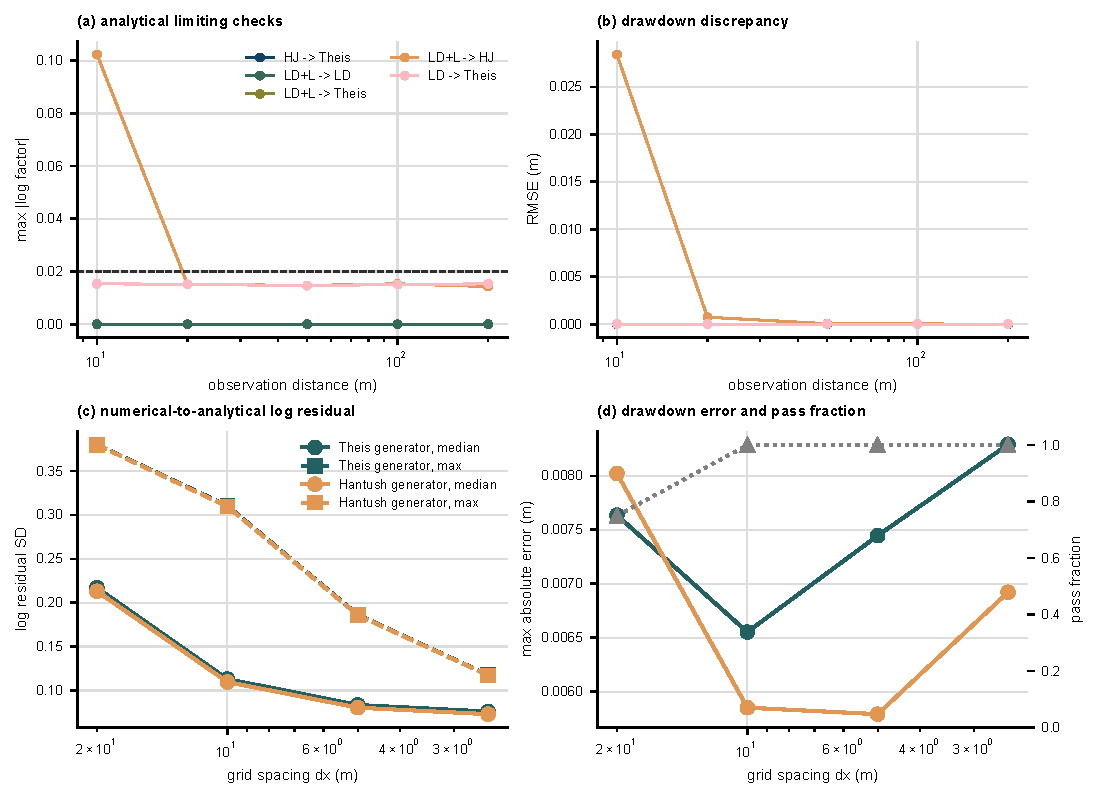
\includegraphics[width=\linewidth]{fig14_mf6_verification_sensitivity.pdf}
\caption{Analytical verification and numerical consistency checks through (a) analytical limit behavior versus observation distance and the dashed log factor tolerance for limit checks; (b) additional analytical limit behavior versus observation distance; (c) numerical consistency with homogeneous Theis analytical reference responses across grid intervals; and (d) numerical consistency with vertical leakage Hantush analytical reference responses across grid intervals. MODFLOW 6 numerical responses and caution labels define finite leakage, near-well, and coarse-grid limits for benchmark scope.}
\label{fig:mf6verification}
\end{figure}

\begin{figure}
\centering
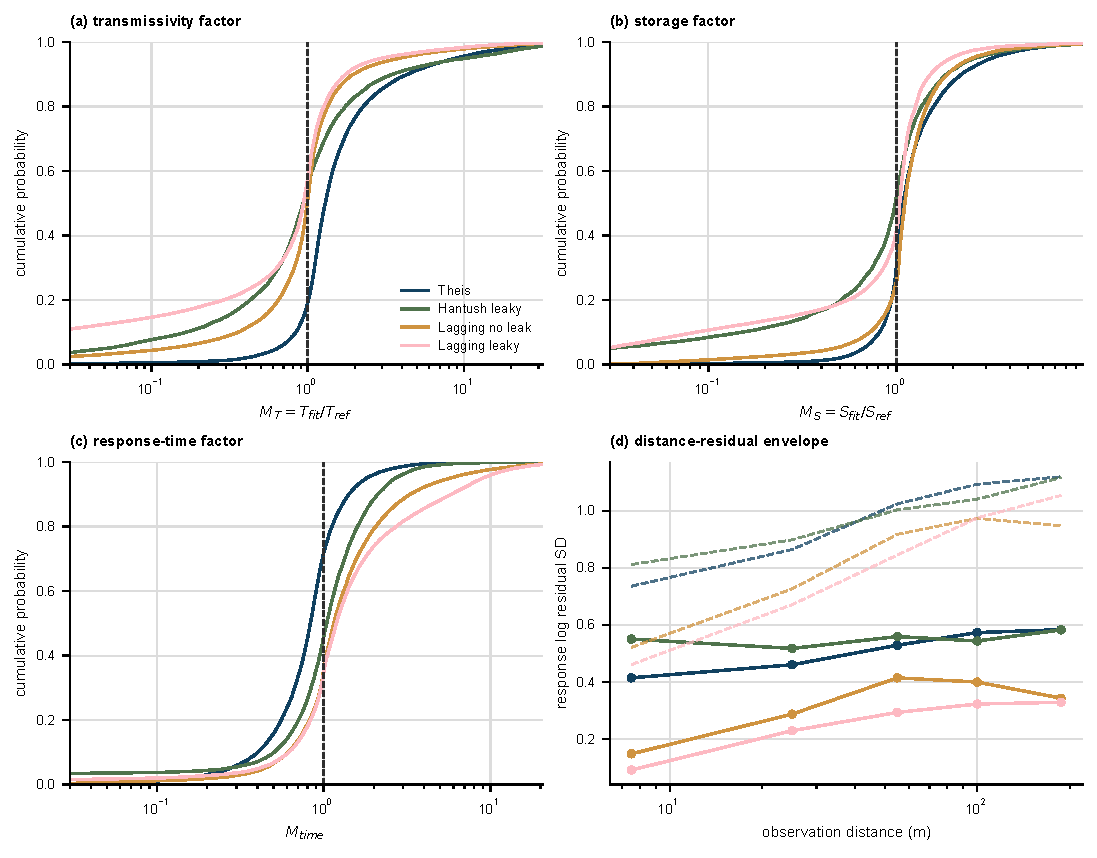
\includegraphics[width=\linewidth]{fig15_mf6_convergence_cov.pdf}
\caption{Screened numerical benchmark model factors through (a) empirical distribution functions for transmissivity model factors after boundary-active fit removal and retention of interpretations within $\Delta BIC \leq 10$; (b) empirical distribution functions for storage model factors under the same screened records; (c) empirical distribution functions for response-time model factors under the same screened records; and (d) median response log residual standard deviation by observation distance, with dashed lines for the 90th percentile envelope. The vertical dashed line in (a)--(c) denotes a factor of one, and all values represent scenario-conditioned model factors for the benchmark classes.}
\label{fig:mf6cov}
\end{figure}

\subsection{Benchmark-conditioned transfer to field diagnostics}

The benchmark-transfer regression connects the controlled benchmark to field use while preserving ambiguity among possible aquifer-process families. Cross validation by complete numerical scenario shows that response diagnostics predict the 90th percentile absolute log model factor with $R^2=0.48$ for transmissivity, $R^2=0.51$ for storage, and $R^2=0.55$ for response time (Figure~\ref{fig:benchmarktransfer}). The strongest predictors are lagging-response residual dispersion, boundary-hit fractions, and BIC preference fractions, indicating that transfer is driven by the same diagnostics used to evaluate the four analytical interpretations.

The field transfer is therefore reported as a model-factor scale across comparable benchmark diagnostics. For Massachusetts, the benchmark transfer gives p90-equivalent model-factor COV values of 0.61 for transmissivity, 0.65 for storage, and 0.90 for response time. For Lovelock Valley, the corresponding values are 0.51, 0.31, and 0.36. These values are smaller than several class-specific conservative COV values in the deterministic applicability table because the regression averages across similar diagnostic behavior in the full numerical ensemble. They are used as benchmark-conditioned sensitivity brackets alongside the deterministic applicability criteria.

\begin{figure}
\centering
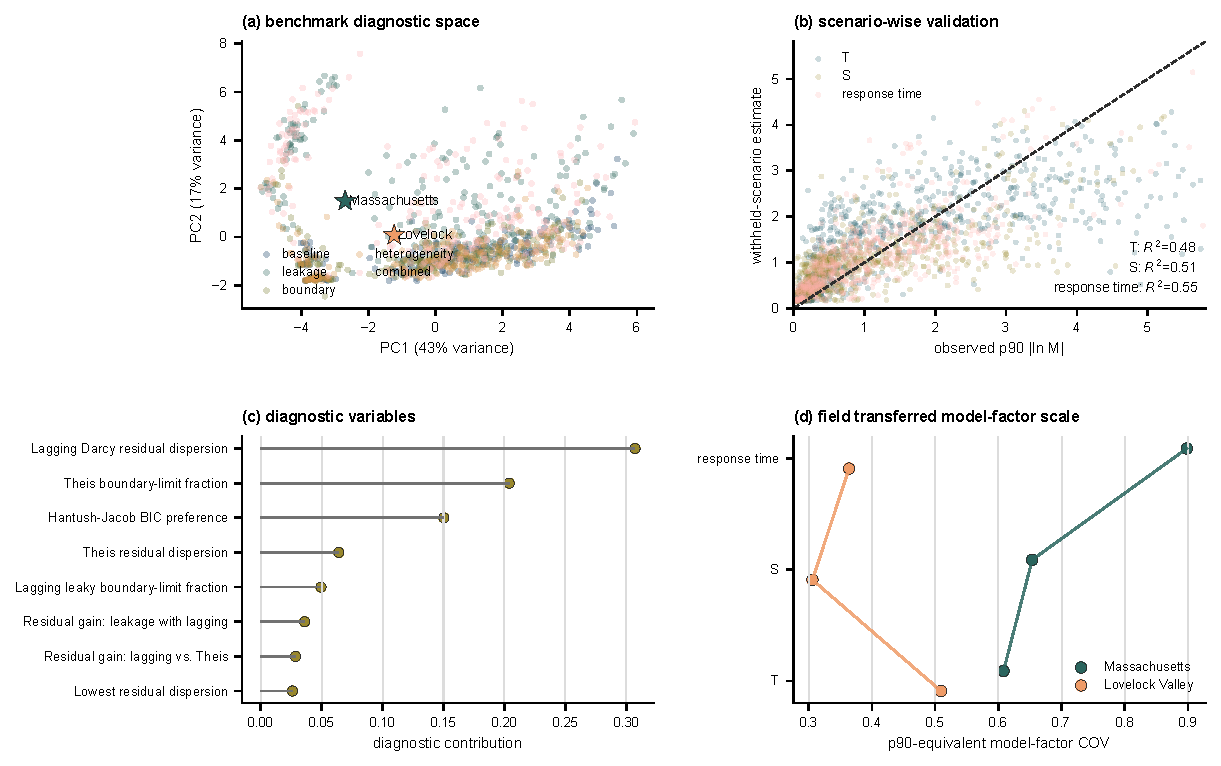
\includegraphics[width=\linewidth]{fig05_benchmark_transfer_layer.pdf}
\caption{Benchmark transfer of aquifer-test transformation uncertainty to field diagnostics through (a) the numerical benchmark response-diagnostic space and the positions of the two field cases; (b) cross-validated predictions versus observed 90th percentile absolute log model factors for transmissivity, storage, and response time; (c) the main diagnostic variables for the regression; and (d) benchmark-transferred, 90th-percentile-equivalent model-factor COV values for the two field cases.}
\label{fig:benchmarktransfer}
\end{figure}

\FloatBarrier

\subsection{Massachusetts diagnostic results}

The field evidence begins with the observation support of the two real cases (Figure~\ref{fig:layout}). Massachusetts observation wells span 5.8--36.6 m from the pumping well and provide 420 retained drawdown observations. Drawdown reproduction provides the primary Massachusetts response evidence: the four interpretation models are overlaid for all 12 observation wells in Figure~\ref{fig:drawdown}.

\begin{figure}
\centering
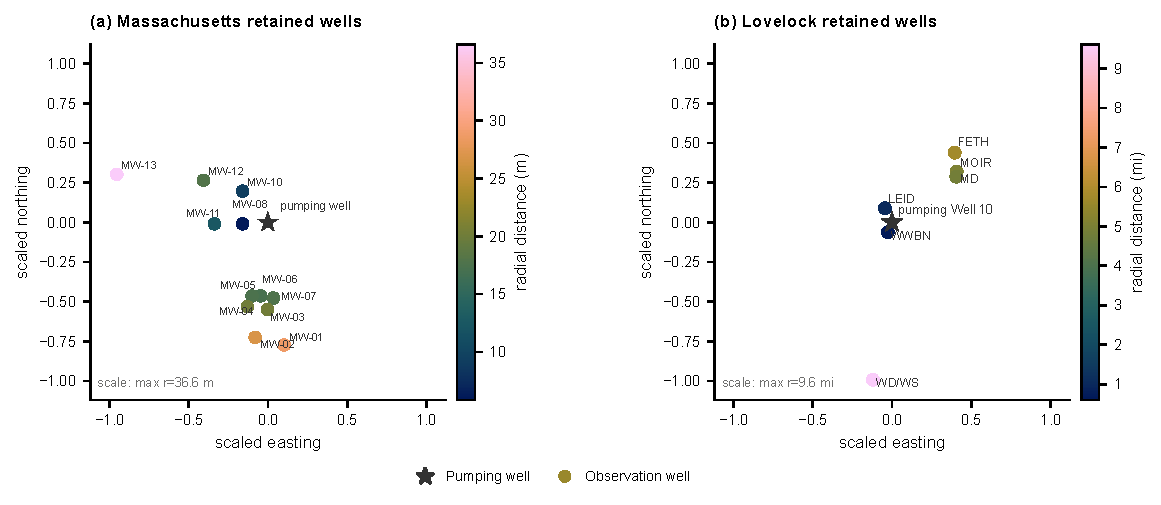
\includegraphics[width=\linewidth]{fig02_site_layout.pdf}
\caption{Paired field-data spatial support for the two real cases through (a) Massachusetts fractured bedrock retained observation wells; and (b) Lovelock Valley MWP2 retained observation wells relative to extraction Well 10. Both panels use coordinates centered on the extraction well and normalized by the maximum retained radial support within the case, so panel shape denotes observation geometry rather than absolute field scale. Circles denote retained observation wells, stars denote extraction wells, and colors retain the actual radial distance within each case.}
\label{fig:layout}
\end{figure}

\begin{figure}
\centering
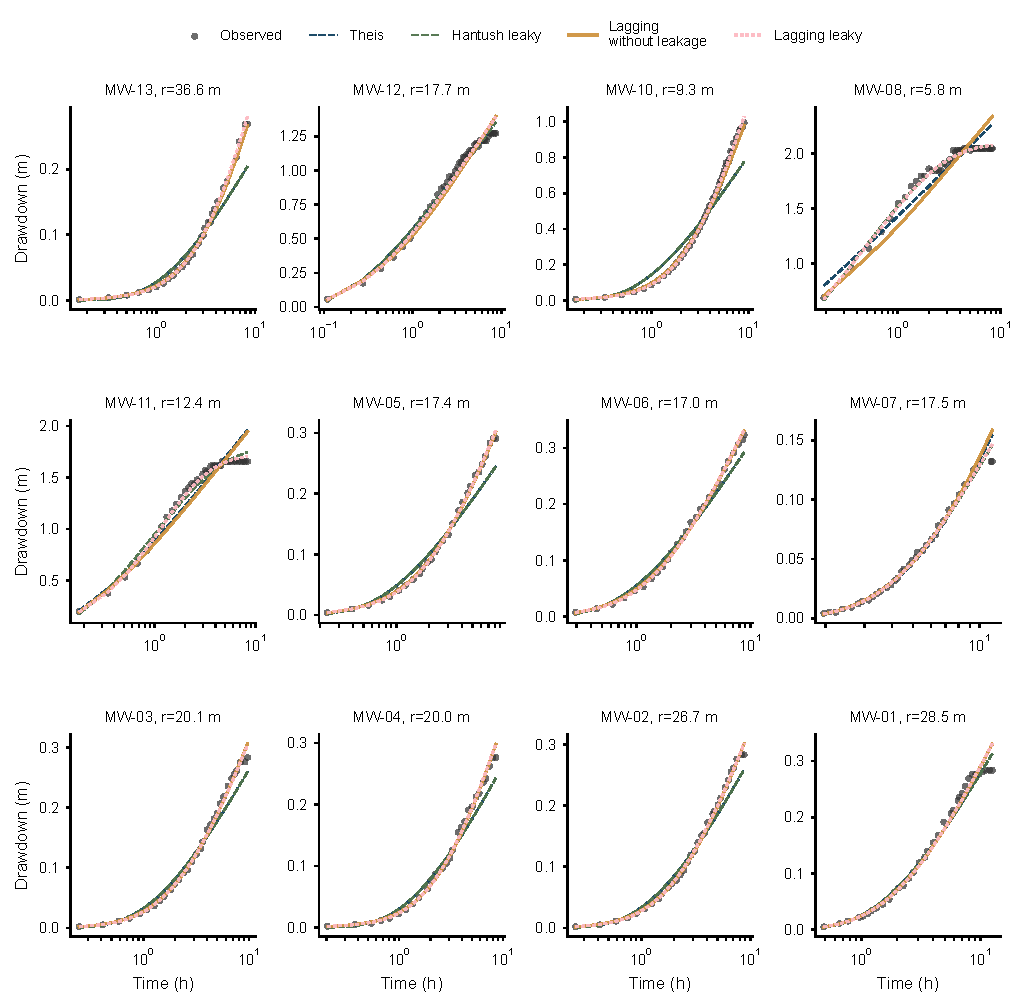
\includegraphics[width=\linewidth]{fig03_observed_simulated_drawdown.pdf}
\caption{Massachusetts observed and simulated drawdown curves for the 12 observation wells across the four main interpretation models, with measured drawdown as points and Theis confined, Hantush--Jacob leaky, lagging Darcy without leakage, and lagging Darcy with leakage predictions as lines.}
\label{fig:drawdown}
\end{figure}

Lagging response terms sharply reduce the Massachusetts log model factor dispersion. Across the four interpretations based on the full observation record, pooled $SD_{\epsilon}$ decreases from 0.166 for Theis confined to 0.164 for Hantush--Jacob leaky, 0.062 for lagging Darcy without leakage, and 0.035 for lagging Darcy with leakage. The largest reduction occurs after the model includes a lagging response term, whereas the leakage term still requires support from complexity and parameter-variability evidence. Observed-predicted scatter and pooled log model factor distribution plots are retained as Supplementary Figures~S1 and S2.

Model complexity and parameter variability qualify this response result (Figure~\ref{fig:variancecov}). BIC prefers lagging Darcy with leakage in 5 of 12 wells, lagging Darcy without leakage in 3 wells, Hantush--Jacob leaky in 2 wells, and Theis confined in 2 wells. The transmissivity COV values are 0.58, 0.78, 0.46, and 0.81, and the storage COV values are 2.05, 1.71, 1.74, and 1.54 for the same model order. Thus, the Massachusetts case supports lagging response as a transformation diagnostic, while the leaky lagging model requires identifiability checks before its additional parameter is interpreted as a field property.

\begin{figure}
\centering
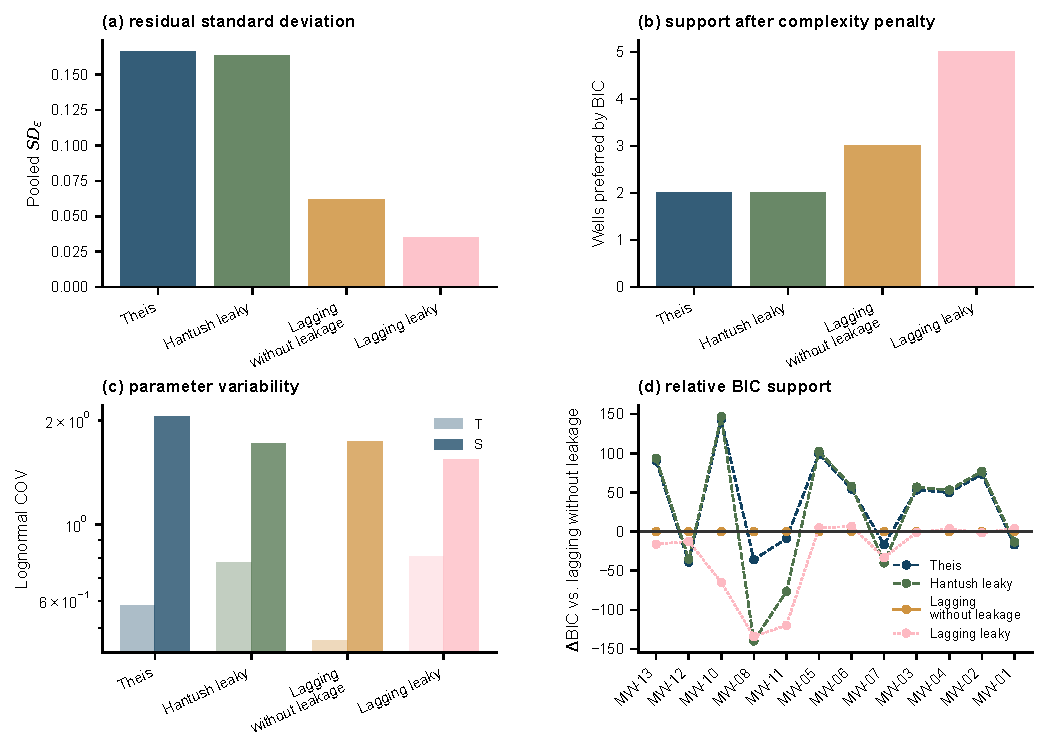
\includegraphics[width=\linewidth]{fig06_massachusetts_pathway_summary.pdf}
\caption{Massachusetts interpretation-model summary through (a) pooled log model factor dispersion; (b) BIC preference counts across the four main interpretation models; (c) lognormal parameter COV for fitted transmissivity and storage; and (d) relative BIC support against lagging Darcy without leakage.}
\label{fig:variancecov}
\end{figure}
\FloatBarrier

\subsection{Lovelock Valley diagnostic results}

Lovelock Valley provides the independent basin fill field case. The retained records include seven observation wells, 520 processed pumping/recovery observations, a larger field support of 0.6--9.6 miles, public observation weights, and a 0.05 ft offset in the log response tied to the report's detection threshold. The Lovelock response curves mirror the Massachusetts drawdown comparison and show fitting at the response level before fitted parameters are interpreted (Figure~\ref{fig:lovelockresponse}).

\begin{figure}
\centering
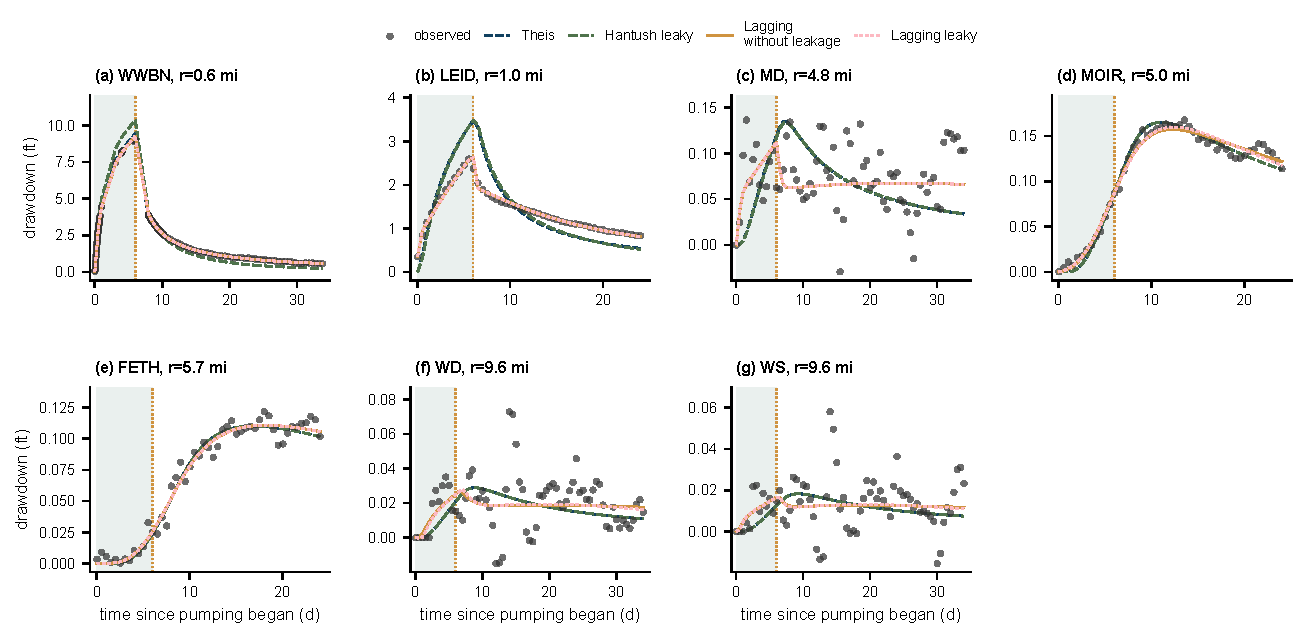
\includegraphics[width=\linewidth]{fig07_lovelock_response_hydrographs.pdf}
\caption{Lovelock Valley MWP2 observed drawdown and recovery responses with fitted curves under the four main interpretation models across seven selected observation wells by distance from Well 10, with measured responses as points, four model predictions as lines, the shaded interval as the extraction period, and the dotted line as shutoff.}
\label{fig:lovelockresponse}
\end{figure}

Lovelock applies the same response-level evidence chain used for Massachusetts. Across the seven selected observation wells, pooled $SD_{\epsilon}$ is 0.246 for Theis confined, 0.294 for Hantush--Jacob leaky, 0.174 for lagging Darcy without leakage, and 0.174 for lagging Darcy with leakage. The log model factor evidence again favors a lagging interpretation, but the leaky model remains indistinguishable from the lagging model without leakage at the response level. The matching observed-predicted scatter and model factor distribution plots are provided as Supplementary Figures~S3 and S4.

Complexity-adjusted Lovelock support is concentrated in interpretations without leakage (Figure~\ref{fig:lovelocksummary}). BIC prefers lagging Darcy without leakage in 5 of 7 wells and Theis confined in 2 of 7 wells. Transmissivity COV values are 3.40, 3.70, 1.83, and 4.77, and storage COV values are 0.89, 0.86, 0.95, and 10.21 in the same model order. Thus, Lovelock supports lagging response structure but provides no complexity-adjusted support for an additional leakage parameter.

\begin{figure}
\centering
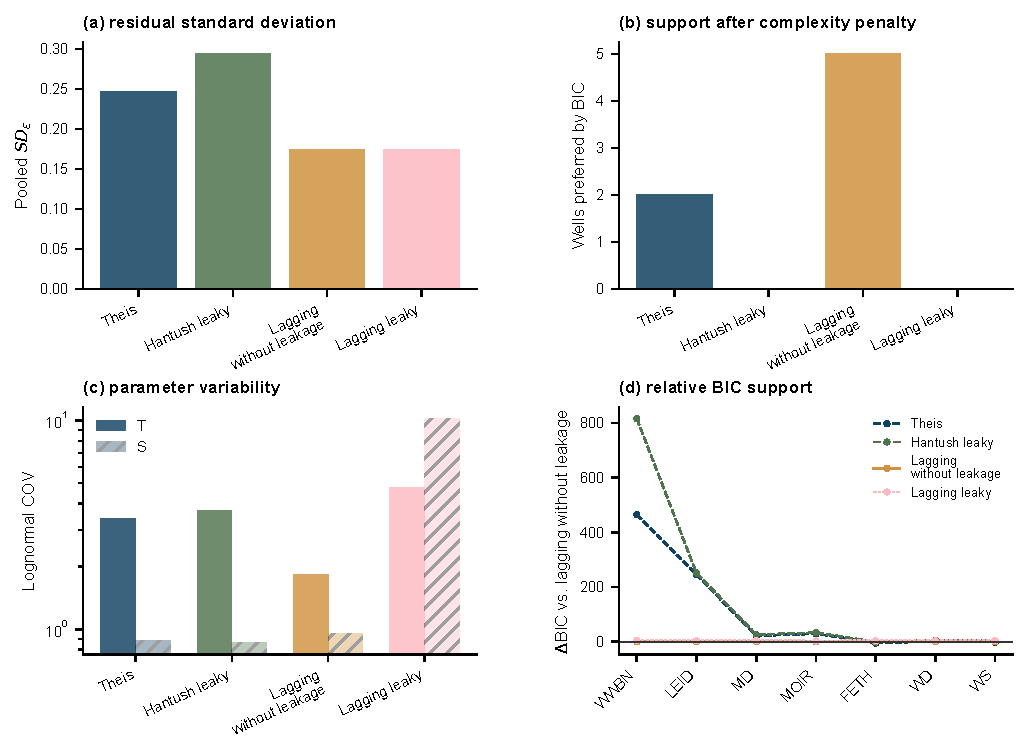
\includegraphics[width=\linewidth]{fig10_lovelock_pathway_summary.pdf}
\caption{Lovelock Valley interpretation-model summary through (a) pooled log model factor dispersion; (b) BIC preference counts across the four main interpretation models; (c) lognormal parameter COV for fitted transmissivity and storage; and (d) relative BIC support against lagging Darcy without leakage.}
\label{fig:lovelocksummary}
\end{figure}
\FloatBarrier

\subsection{Synthesis of the two field cases and scope of inference}

The two field cases show parallel response evidence but different leakage support. Massachusetts represents a small fractured bedrock drawdown subset with 12 wells, 420 retained observations, and 5.8--36.6 m radial support. Lovelock Valley represents a larger basin fill pumping/recovery case with seven retained observation wells, 520 processed observations, 0.6--9.6 mi radial support, and public weights tied to the report's detection threshold. In the common Theis / Hantush--Jacob / lagging Darcy without leakage / lagging Darcy with leakage order, Massachusetts gives $SD_{\epsilon}$ = 0.166 / 0.164 / 0.062 / 0.035, BIC preferred wells = 2 / 2 / 3 / 5, and transmissivity COV = 0.58 / 0.78 / 0.46 / 0.81; Lovelock Valley gives $SD_{\epsilon}$ = 0.246 / 0.294 / 0.174 / 0.174, BIC preferred wells = 2 / 0 / 5 / 0, and transmissivity COV = 3.40 / 3.70 / 1.83 / 4.77. The full four-model headline table, including storage COV and validation scope, is provided in Supplementary Table~S2.

The final synthesis identifies transformation uncertainty as a reporting issue in aquifer test interpretation (Figure~\ref{fig:fieldexternal}). In both field cases, the lagging interpretation reduces log model factor dispersion relative to the classical confined reference. Direct geological interpretation of additional fitted parameters requires the accompanying diagnostics for response support, complexity support, parameter spread, and validation scope. Fitted transmissivity and storage should therefore be reported with the interpretation model, log model factor dispersion, complexity support, parameter spread, and the scope of validation for each case.

\begin{figure}
\centering
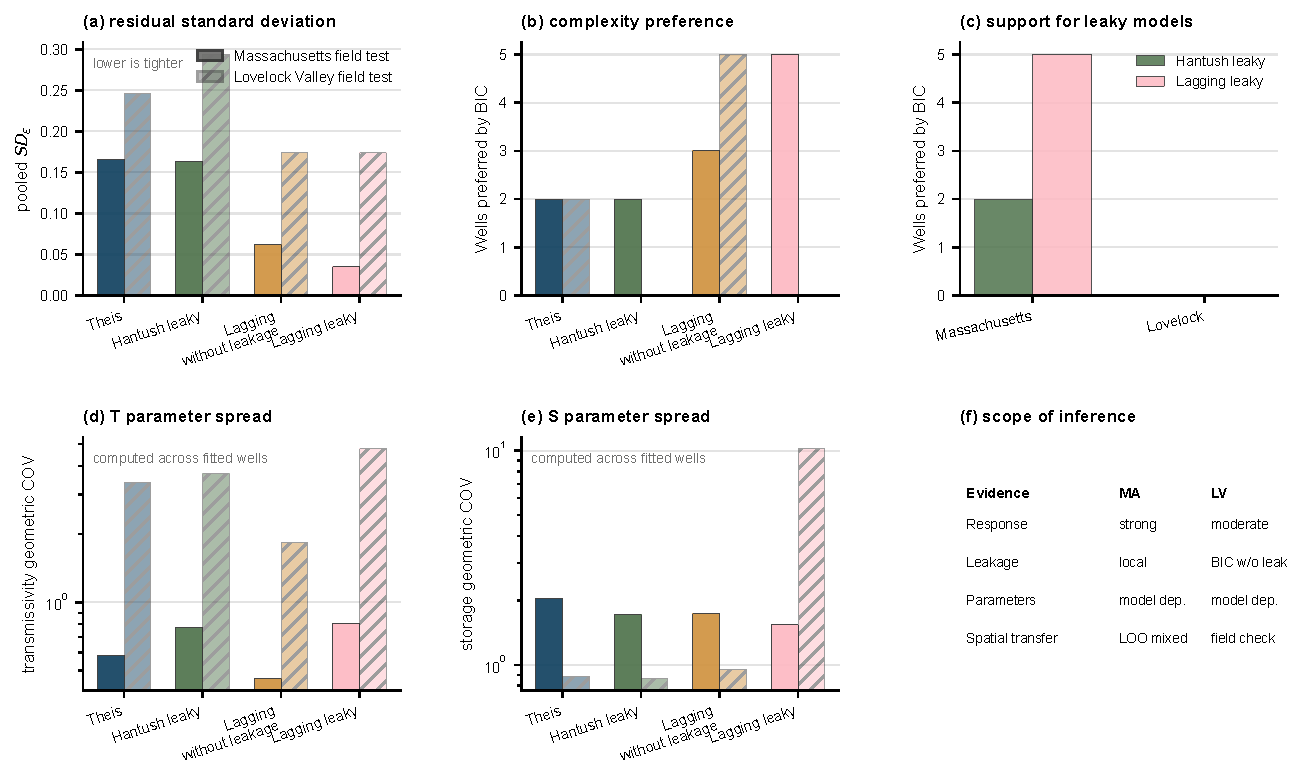
\includegraphics[width=\linewidth]{fig11_two_case_synthesis.pdf}
\caption{Validation synthesis from the Massachusetts fractured bedrock case and the Lovelock Valley basin-fill case through (a) pooled log model factor dispersion; (b) BIC preference counts by well; (c) support for leakage-inclusive models; (d) transmissivity COV; (e) storage COV; and (f) inference scope across response support, leakage support, parameter interpretation, and spatial transfer availability.}
\label{fig:fieldexternal}
\end{figure}

After the two field evidence chains are established, field applicability screening links the field diagnostics back to the numerical benchmark classes (Figure~\ref{fig:mf6fieldapp}). Massachusetts maps primarily to the combined leakage and boundary class, with heterogeneous leakage, heterogeneous boundary, and heterogeneous hydraulic conductivity classes retained as sensitivity or lower complexity checks. Lovelock Valley maps primarily to heterogeneous storage and heterogeneous hydraulic conductivity classes, while heterogeneous leakage is retained only as a local leakage sensitivity because BIC support concentrates in no leakage interpretations. These criteria define where benchmark model factors can inform field interpretation for each site.

\begin{figure}
\centering
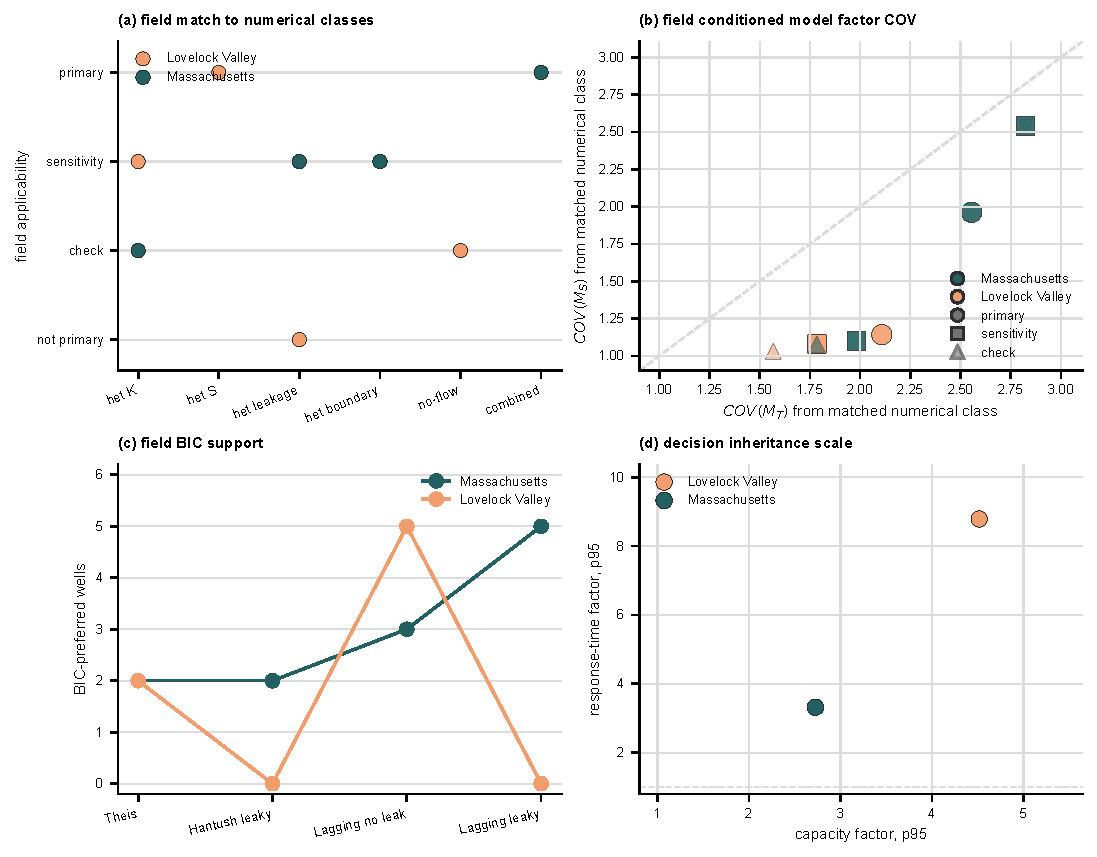
\includegraphics[width=\linewidth]{fig16_mf6_field_applicability.pdf}
\caption{Field application of scenario-conditioned transformation model factors after field evidence-chain establishment through (a) assignment of the two field cases to numerical benchmark classes and applicability levels; (b) matched transmissivity and storage model factor COV values as field sensitivity brackets or conservative priors; (c) field BIC support for the four analytical interpretations; and (d) inherited 95th percentile capacity and response-time factors from the model-averaged decision diagnostic. The figure identifies where benchmark factors enter the field interpretation.}
\label{fig:mf6fieldapp}
\end{figure}
\FloatBarrier

\subsection{Management consequence of aquifer test transformation uncertainty}

The model averaged management diagnostic carries the four aquifer test interpretations into a BMA distribution upstream of a site-scale groundwater model. Figure~\ref{fig:decisionconsequence} reports decision quantities derived from the same fitted $T$ and $S$ values, and Supplementary Table~S3 gives the numerical table. Strict BIC weights represent single-model reporting when the information criterion concentrates support on one interpretation. Variance window weights retain plausible alternatives by normalizing BIC differences by the well specific BIC spread.

The result shows why the engineering consequence is better expressed through transmissivity, hydraulic diffusivity, and response time. Under strict BIC weights, the median robust hydraulic control capacity factor is 1.00 in both field cases, reflecting the near single model behavior of the posterior weights. Under variance window weights, the median capacity factor increases to 1.60 in Massachusetts and 1.18 in Lovelock Valley, with 95th percentile factors of 2.73 and 4.52. The corresponding mean probability that the selected interpretation underestimates hydraulic control capacity is 0.38 in Massachusetts and 0.21 in Lovelock Valley.

The response time consequence is also larger than the observation-scale drawdown difference. Under variance window weights, the median response time factor is 1.85 in Massachusetts and 4.05 in Lovelock Valley, with 95th percentile factors of 3.32 and 8.79. The mean probability that the BMA mixture contains a faster response than the selected interpretation is 0.41 and 0.23. These values are aquifer-test inheritance diagnostics rather than project failure probabilities because they are computed from interpretation models rather than a project specific MODFLOW management model. They show what a later groundwater control or management calculation can inherit if a pumping test report provides one selected $T$ and $S$ without documenting interpretation model uncertainty.

The model weights also show that the decision diagnostic is not driven by always selecting the most complex interpretation. Massachusetts gives nonzero variance window support to all four interpretations, with the largest mean weight on lagging Darcy with leakage. Lovelock Valley assigns the largest mean weight to lagging Darcy without leakage, but Theis and lagging with leakage both retain nontrivial support. The diagnostic therefore uses the field supported mixture in each case rather than forcing the same preferred interpretation onto both sites. The key inheritance problem is that strict single-model reporting can make the aquifer test input look sufficiently certain even when alternative formal interpretations would change capacity or response time decisions by factors of two to nine.

\begin{figure}
\centering
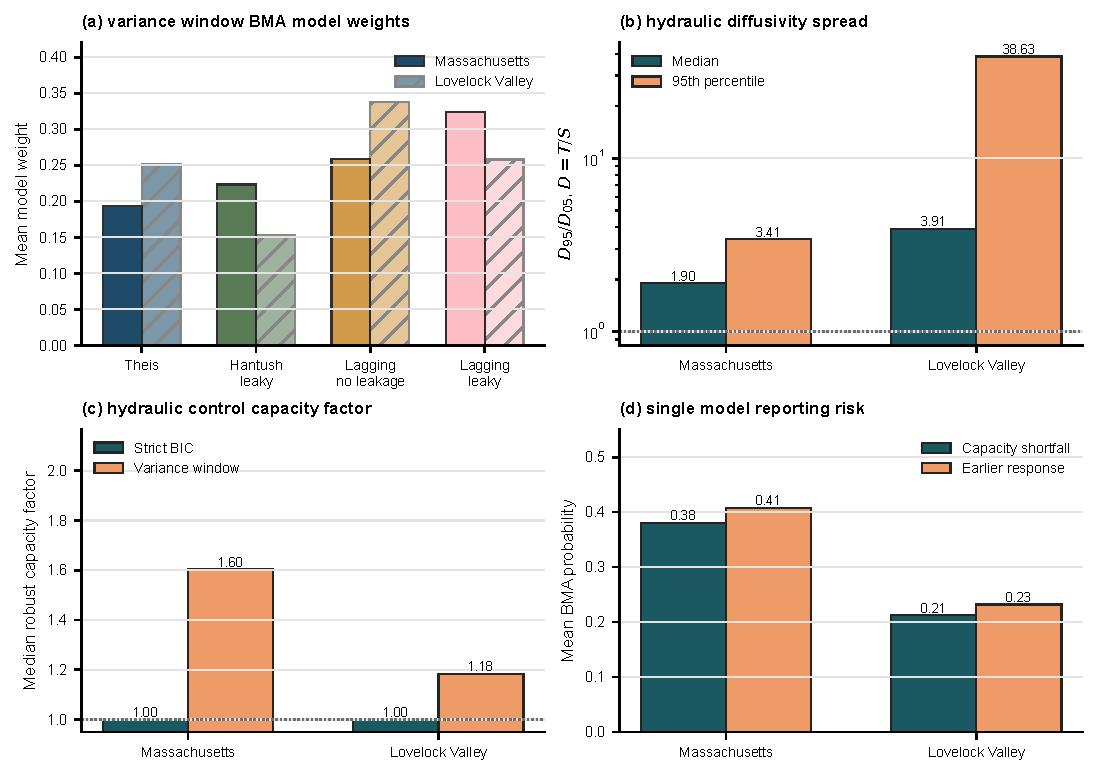
\includegraphics[width=\linewidth]{fig12_decision_consequence.pdf}
\caption{Model-averaged propagation of aquifer-test interpretation uncertainty to management-relevant hydraulic quantities through (a) mean variance-window BMA weights for the four analytical interpretations; (b) median and 95th percentile hydraulic diffusivity spread, expressed as $D_{95}/D_{05}$ with $D=T/S$; (c) median robust hydraulic control capacity factor under strict BIC weights and variance-window weights; and (d) mean variance-window BMA probability of selected-interpretation underestimation of hydraulic control capacity or missed earlier hydraulic response.}
\label{fig:decisionconsequence}
\end{figure}

\subsection{Implications for groundwater uncertainty analysis}

Aquifer test parameters used in groundwater models and management calculations depend on the interpretation model that converts drawdown to fitted values. That transformation changes both the log model factor in the response and the inferred parameter field. The evidence therefore combines controlled numerical checks under prescribed aquifer conditions, log model factor dispersion, information criteria, parameter variability, leakage support, field case limitations, and two-case consistency. The numerical benchmark tests recovery and model factor calibration where the aquifer conditions are controlled by design. Site specific field diagnostics support local interpretation, while the cross-case inference rests on evidence that appears in both field cases. The resulting reporting endpoint is to state the measured response support, interpretation model, response log model factor, complexity support, parameter spread, numerical benchmark match, field applicability screening, and decision consequence before pumping-test-derived hydraulic properties are used; the full checklist is given in Supplementary Table~S4.

The reporting structure addresses a central groundwater interpretation risk. If model-form error is hidden inside fitted transmissivity and storage values, later groundwater flow models, capture analyses, dewatering calculations, or allocation studies may treat transformation error as site heterogeneity. Reporting the log model factor, the complexity-adjusted support, the inferred parameter spread, and the validation scope makes that distinction explicit. These diagnostics define a stricter standard for deciding when aquifer test parameters are ready to support groundwater interpretation.

\subsection{Lagging Darcy as a diagnostic tool}

The lagging Darcy interpretations reduce log model factor dispersion. This reduction directly addresses the transformation uncertainty term in Equation~\ref{eq:aquifer_transform} because $SD_{\epsilon}$ is the group dispersion of $\eta_{M,i,j}$ defined in Equation~\ref{eq:sd_epsilon}. The classical transformation without lag leaves a systematic response mismatch, making the log model factor structure a signal from the interpretation model before inverse algorithms treat it as aquifer heterogeneity. Lagging Darcy therefore serves as a diagnostic interpretation for nonsteady response structure within the broader set of established aquifer test interpretations. Its no-leakage and leaky forms separate two questions: whether temporal memory is needed, and whether leakage is supported strongly enough to justify a finite $B$. Groundwater flow models, risk assessments, and engineering calculations frequently inherit $T$ and $S$ values from aquifer test interpretations; if response mismatches introduced by the model remain hidden inside those inferred parameters, later spatial analyses may interpret transformation error as hydrogeologic heterogeneity.

\subsection{Leakage and first type boundary alternatives}

The diagnostic for late time flattening remains important because it tests conventional explanations alongside lagging behavior. Hantush--Jacob leakage and a first type constant head boundary can both flatten drawdown at late time, while Theis retains the familiar confined aquifer reference interpretation. In the Massachusetts case, auxiliary checks indicate selective leakage or behavior equivalent to a boundary, with support concentrated in specific wells. In the Lovelock case, BIC preference is concentrated in interpretations without leakage. The result across cases supports treating leakage as an explicit competing interpretation before fitted storage and transmissivity are interpreted as direct evidence of aquifer heterogeneity.

The methodological implication is that leakage and boundary alternatives should remain explicit candidates. The original lagging leaky model is represented in the field comparison, and the leakage factor carries interpretive value when it is identifiable and improves the field evidence. The comparison therefore treats lagging with leakage as a more demanding interpretation than the lagging interpretation without leakage.

\subsection{Why response improvement and parameter convergence differ}

The inferred parameters place the response improvement in context. Lagging Darcy reduces log model factor dispersion, but parameter convergence is weaker and differs by site. This pattern aligns with aquifer test studies showing that drawdown-inferred parameters often behave as apparent or effective quantities, with transmissivity and storage responding differently to heterogeneity, observation geometry, and model form \citep{sanchez_vila1999,manewell2022}. The central diagnostic result is this contrast between response fit and parameter interpretation. A model can reproduce drawdown more accurately while redistributing uncertainty among $S$, $T$, $B$, $\tau_q$, and $\tau_s$. Lagging Darcy reports should include log model factor dispersion, information criteria, parameter COV, leakage support, and the validation scope supported by the available field design.

The Lovelock field case reinforces this distinction under a separate basin fill pumping/recovery design. Its smaller reduction in response variance likely reflects differences in site scale, preprocessing, environmental correction, observation weighting, and the regional pumping/recovery design. The parallel diagnostic display interprets Lovelock using the same log model factor dispersion, model factor distribution, BIC support, and parameter-variability metrics used for Massachusetts. The evidence direction remains consistent: lagging Darcy reduces log model factor dispersion and remains competitive after model complexity penalties, while storage and transmissivity do not converge uniformly. This case shows that unresolved temporal response structures remain visible across contrasting field settings and materially change inferred parameter values.

\subsection{Relation to stochastic hydrogeology and model uncertainty}

The proposed interpretation analysis complements stochastic hydrogeology and groundwater model uncertainty analysis rather than replacing them. Random field models and Monte Carlo simulations remain appropriate for propagating spatial heterogeneity through groundwater predictions \citep{dagan1989,gelhar1993,rubin2003}. Multimodel approaches remain appropriate when several plausible conceptual models require integration into predictions \citep{poeter_anderson2005,rojas2008,ye2010}. Broader groundwater uncertainty frameworks address model structure error, hydrostratigraphic alternatives, conceptual model propositions, data worth, management forecasts, and model structural adequacy \citep{refsgaard2006,li_tsai2009,tsai2010,tsai_elshall2013,guillaume2016,fienen2025}. The present work examines the preceding interpretation step: the uncertainty introduced by drawdown-to-parameter interpretation before investigators build a spatial field, model ensemble, or management forecast.

Adjacent groundwater studies already address several downstream or support-scale questions. Beckie and Harvey \citep{beckie_harvey2002} show that a slug test can be interpreted as a weighted support average. Manewell, Doherty, and Hayes \citep{manewell2022,manewell2024} examine how aquifer test interpretations can be incorporated into groundwater model parameterization. Naderi and Gupta \citep{naderi_gupta2023} define requirements for inferring aquifer-scale transmissivity and storage in heterogeneous confined aquifers. Li and Tsai \citep{li_tsai2009}, Tsai \citep{tsai2010}, and Tsai and Elshall \citep{tsai_elshall2013} treat multimodel and hierarchical uncertainty after groundwater model alternatives have been specified. The present procedure is placed before those downstream analyses. It evaluates whether the parameters handed to them already carry unresolved interpretation dependence.

The 10,000 controlled scenarios sharpen this distinction before the field cases are used. Response residuals, parameter model factors, and decision model factors do not have the same controlling drivers. Within the screened records, response residual standard deviation is dominated by water-level noise and observation support, whereas transmissivity and storage model factors remain strongly interpretation dependent. This behavior is important for BMA and groundwater management calculations. BMA can combine candidate predictions and separate uncertainty components, but the spread available to that calculation depends on the aquifer-test inputs supplied to it. The present diagnostic therefore propagates the four analytical interpretations into $T$, $D=T/S$, and $t_c \propto S/T$. Under variance window BMA, the selected interpretation can understate hydraulic control capacity by factors of 1.60 and 1.18 at the median, and response time can be optimistic by factors of 1.85 and 4.05. Later uncertainty propagation may therefore become overconfident if transmissivity and storage enter a numerical model as deterministic values, tight priors, or calibration labels without recording the interpretation model, log model factor, benchmark model factors, and field-to-benchmark applicability criteria. The proposed reporting structure improves traceability by linking measured drawdown, interpretation model, response-level log model factor, parameter spread, numerical model factor calibration, model averaged management diagnostic, and the decision quantity that inherits the parameter.

\subsection{Scope of inference from field data}

The two field cases define both the value and the scope of the study. The Massachusetts and Lovelock tests show that unresolved temporal response structure can materially change fitted responses and inferred parameters across contrasting geological settings. The numerical benchmark results provide conditional external model factors for selected scenario classes, while independent recovery of true field transmissivity, storage, leakage factor, or lagging response times would require additional field constraints at the support scale. The analytical and numerical consistency warnings also define practical limits: near well finite leakage behavior and coarse grid spacing require additional checks before supporting strong field parameter claims. Lagging Darcy is therefore treated as one candidate interpretation family, while Theis, Hantush--Jacob leaky, and boundary diagnostics remain competing conventional references.

The field response improvement establishes a diagnostic role for lagging Darcy within broader aquifer-test interpretation. Project design use requires the same evidence demanded of conventional interpretations: independent constraints, blocked predictive validation, no major identifiability failure, and decision propagation for the specific project. The field cases reach a diagnostic standard and define the evidence needed before project specific design use.

\subsection{Groundwater calculation inheritance}

The practical contribution is a reporting procedure for groundwater use of aquifer test parameters. Estimates from pumping tests commonly enter groundwater flow models, capture analyses, dewatering designs, contaminant control evaluations, and groundwater allocation studies as fixed input parameters. The results indicate that reports should state the interpretation model, log model factor dispersion, support from information criteria, variability in inferred hydraulic properties, leakage or boundary alternatives when supported, and the supported scope of validation before treating fitted transmissivity and storage values as direct evidence of subsurface heterogeneity. This distinction supports defensible parameter selection and uncertainty communication when water resource decisions depend on groundwater response predictions.

The procedure is relevant when groundwater boundary conditions, pumping demands, or recharge conditions may change over a management or project horizon. Groundwater control and management problems often ask how much pumping capacity is needed and how quickly hydraulic response reaches monitoring points, supply wells, stream boundaries, or sensitive receptors. In those calculations, the relevant inherited quantities are not only drawdown residuals; they are $T$, $S$, $T/S$, and $S/T$. The model averaged diagnostic gives this effect a practical scale. Under variance window BMA, the 95th percentile robust capacity factor reaches 2.73 in Massachusetts and 4.52 in Lovelock Valley, and the 95th percentile response time factor reaches 3.32 and 8.79. The result defines an applicability check for later project specific optimization or management models: the pumping test report should document whether the selected interpretation leaves enough transformation uncertainty to alter the capacity or timing variables inherited by later groundwater calculations.

The field cases and numerical benchmark identify the set of diagnostics needed before propagating aquifer test parameters to a project specific dewatering, capture, saltwater intrusion, streamflow depletion, or groundwater allocation model: log model factor dispersion, complexity support, parameter spread, leakage or boundary alternatives, scenario-conditioned model factor COV, scope of validation, model averaged management diagnostic, and the interpretation model used to estimate apparent aquifer properties from measured drawdown.

\subsection{Scope of the evidence}

The evidence supports five conclusions. Pumping test interpretation can introduce transformation uncertainty before transmissivity and storage are propagated. The response-level log model factor quantifies interpretation-dependent residual structure. Controlled numerical scenarios estimate conditional parameter model factor bias and COV for specified aquifer classes. Apparent variability in transmissivity and storage is partly dependent on the interpretation model. The model averaged diagnostic shows that this interpretation dependence can propagate to management-relevant hydraulic quantities.

The present results support lagging Darcy as a diagnostic interpretation family within a broader set of conventional aquifer-test solutions. They complement existing groundwater uncertainty methods by examining the preceding drawdown-to-parameter conversion. Field data alone provide response diagnostics under specified observation supports; the numerical benchmark supplies the scenario-conditioned controlled checks used to interpret parameter model factors.

\subsection{Limitations}

The field demonstration has a defined scope. The Massachusetts results derive from one retained constant rate subset of a fractured bedrock pumping test with 12 wells, and the Lovelock case provides an independent field comparison with different preprocessing, observation weighting, and support. The reported field COV values are specific to these test systems. The numerical benchmark model factor COV values are conditional on the scenario class, support definition, observation geometry, pumping schedule, grid design, screening criteria, and four implemented analytical interpretations. Their use as transformation priors is appropriate when field diagnostics support a comparable class. Direct evaluation of field parameter recovery would require independent reference values for $T$, $S$, $B$, $r_I$, $\tau_q$, and $\tau_s$. Evaluation of the full second moment decomposition in Equation~\ref{eq:second_moment} would also require complete measurement budgets for water levels, pumping rates, distances, aquifer thicknesses, and the simplification of the Massachusetts pumping history with variable rates.

The model averaged management analysis uses fitted aquifer test parameters and analytical decision indices to define an inheritance diagnostic for later groundwater calculations. Project specific groundwater management models, capture zone analyses, or optimization studies would provide the next level of decision support. The variance window weights are a sensitivity diagnostic and should be read alongside the strict BIC weights rather than as a unique posterior probability claim. The final MAP refit uses weak lognormal prior residuals, so the lagging time and leakage estimates are regularized diagnostic response quantities in the current field evidence. Several lagging leaky fits approach the upper bound for inactive leakage in $B$, indicating weak identifiability of the leakage factor in those wells. The local MAP covariance diagnostic relies on a quadratic approximation around the fitted optima. The Hantush--Jacob and constant head boundary fits represent diagnostic equivalent interpretations of leakage or boundary behavior. The validation that excludes one well at a time operates as a diagnostic for spatial transfer in the Massachusetts case, while the Lovelock data provide the independent field consistency check.

The benchmark-transfer analysis is bounded by the numerical design. Its validation supports prediction of model-factor magnitude better than unique scenario identification, so the transferred COV values are reported as benchmark-conditioned sensitivity brackets for field diagnostics represented by the benchmark.

Future work should add independent reference tests and broader model families, including delayed yield, wellbore storage and skin, generalized radial flow, dual porosity, exchange between fractures and matrix, unconfined numerical benchmarks, and heterogeneous numerical inverse models. Those additions would strengthen the current field evidence through explicit support criteria, blocked validation designs, profile likelihood or posterior checks, and propagation to dewatering, capture, saltwater intrusion, or groundwater allocation criteria for specific projects.

\section{Conclusions}

The analysis establishes a benchmark-conditioned framework for tracing how aquifer-test drawdown becomes inferred groundwater parameters. The framework separates measured response, four analytical transformations, response-level log model factors, support-matched numerical reference values, benchmark model-factor magnitude, field transfer diagnostics, and decision quantities inherited by later groundwater calculations. This sequence shifts the uncertainty problem upstream of conventional stochastic groundwater modeling: transmissivity and storage enter later models as interpreted quantities, not direct observations.

The 10,000 scenario numerical benchmark provides the controlled reference basis. It produced 160,012 fitted interpretation and well records across homogeneous, leaky, finite-boundary, heterogeneous, and combined settings. Analytical limiting checks confirmed physical consistency in 22 of 25 cases, and numerical consistency checks aligned with analytical reference responses in 30 of 32 configurations. The screened benchmark showed that response fit, parameter recovery, and decision-factor propagation are distinct quantities; across class and interpretation groups in the screened records, median model-factor COV values were 2.06 for transmissivity, 1.27 for storage, and 1.21 for response time.

The benchmark-transfer analysis links that controlled benchmark to field diagnostics while preserving ambiguity among possible aquifer-process families. Nonlinear regression ensembles by complete numerical scenario predicted the 90th percentile absolute log model factor with cross-validated $R^2$ values of 0.48, 0.51, and 0.55 for transmissivity, storage, and response time. Applying the same response diagnostics to the field cases gave p90-equivalent benchmark-transferred model-factor COV values of 0.61--0.90 for Massachusetts and 0.31--0.51 for Lovelock Valley. These values are sensitivity brackets conditioned on the represented benchmark diagnostics.

The two field cases demonstrate how the benchmark-conditioned framework changes aquifer-test reporting. In Massachusetts, pooled log model factor dispersion decreased from 0.166 for Theis confined to 0.062 for lagging Darcy without leakage and 0.035 for lagging Darcy with leakage. In Lovelock Valley, dispersion decreased from 0.246 for Theis confined to approximately 0.174 for the two lagging interpretations, while BIC support concentrated in the no-leakage lagging form. These results support lagging Darcy as a useful diagnostic interpretation for unresolved temporal response structure within a broader set of conventional pumping-test solutions.

The model-averaged management diagnostic shows why the upstream drawdown-to-parameter conversion matters for groundwater calculations. Under variance window weighting of the four formal interpretations, the median robust hydraulic control capacity factor was 1.60 in Massachusetts and 1.18 in Lovelock Valley, with 95th percentile factors of 2.73 and 4.52. The median response-time factor was 1.85 and 4.05, with 95th percentile factors of 3.32 and 8.79. Aquifer-test reports should therefore state the interpretation model, response residual structure, benchmark transfer support, parameter spread, validation scope, and inherited decision consequence before fitted parameters are treated as direct hydrogeologic evidence or deterministic groundwater model inputs.

\section*{Acknowledgments}

YFL thanks the John Su Foundation for its support.

\section*{Nomenclature}

\begingroup
\scriptsize
\setlength{\tabcolsep}{3pt}
\renewcommand{\arraystretch}{0.86}
\begin{longtable}{@{}p{0.18\linewidth}p{0.68\linewidth}@{}}
    \toprule
    Symbol & Meaning \\
    \midrule
    \endhead
    $S$ & Storage coefficient inferred from pumping test interpretation \\
    $T$ & Transmissivity inferred from pumping test interpretation \\
    $B$ & Leakage factor in the Hantush--Jacob or lagging leaky interpretation \\
    $r_I$ & Effective image well distance in the constant head boundary diagnostic \\
    $\tau_q$ & Diagnostic flux gradient lag time in the lagging Darcy interpretation \\
    $\tau_s$ & Diagnostic storage release lag time in the lagging Darcy interpretation \\
    $\epsilon$ & Transformation uncertainty or residual component in the response model \\
    $c$ & Case specific positive offset used in the log response transformation \\
    $G$ & Diagnostic group of observations, such as full record, well, field case, or time window \\
    $z_{\mathrm{obs},i,j}$, $z_{M,i,j}$ & Observed and modeled log responses for well $i$ and time $j$ \\
    $\eta_{M,i,j}$ & Log model factor for interpretation model $M$, well $i$, and observation time $j$ \\
    $\widehat{F}_{\eta,M}$ & Empirical distribution of the log model factor for interpretation model $M$ \\
    $F_{M,i,j}$ & Multiplicative model factor, equal to $\exp(\eta_{M,i,j})$ \\
    $M_{T,M}$, $M_{S,M}$ & Numerical benchmark parameter model factors for transmissivity and storage under interpretation model $M$ \\
    $T_{\mathrm{app},M}$, $S_{\mathrm{app},M}$ & Apparent transmissivity and storage inferred by interpretation model $M$ \\
    $T_{\mathrm{ref}}$, $S_{\mathrm{ref}}$ & Support-matched reference transmissivity and storage in the numerical benchmark \\
    $COV_M$ & Coefficient of variation of a lognormal model factor computed from $\sigma_{\ln M}$ \\
    $w_{M,i}$ & BIC posterior weight for interpretation model $M$ in field case or well group $i$ \\
    $w^{V}_{M,i}$ & Variance window BMA weight for interpretation model $M$ \\
    $\Delta BIC_{M,i}$ & Difference between model $M$ and the minimum BIC value for well or group $i$ \\
    $s_{\Delta BIC,i}$ & Standard deviation of the four $\Delta BIC$ values used in the variance window weight \\
    $x_{M,i}$ & Model-derived decision variable entering the model averaged management diagnostic \\
    $D_{M,i}$ & Hydraulic diffusivity, equal to $T_{M,i}/S_{M,i}$ \\
    $t_{c,M,i}$ & Characteristic response time proportional to $S_{M,i}/T_{M,i}$ at distance $r_i$ \\
    $M_i^*$ & Selected interpretation under the variance window BMA weight \\
    $R^C_i$ & Robust hydraulic control capacity factor relative to the selected interpretation \\
    $P^C_i$ & Probability that the selected interpretation underestimates hydraulic control capacity \\
    $R^t_i$ & Response time factor relative to the selected interpretation \\
    $P^t_i$ & Probability that the BMA mixture contains a faster response than the selected interpretation \\
    $SD_{\epsilon}$ & Standard deviation of the log model factor in a diagnostic group \\
    $COV_{F,M}$ & Lognormal coefficient of variation for the multiplicative response model factor \\
    $VR_{\epsilon}$ & Response variance ratio between lagging and classical transformations \\
    $\xi_d$ & Derived or design property produced by a transformation model \\
    $\xi_m$ & Measured property or measured response entering a transformation model \\
    $\mathbf{y}_{m,i}$ & Measured pumping test vector for observation well $i$ \\
    $\boldsymbol{\theta}_{M,i}$ & Parameter vector inferred by interpretation model $M$ for well $i$ \\
    $\mathcal{T}$, $\mathcal{T}_M$ & Generic transformation function and interpretation transformation associated with model $M$ \\
    $COV_X$ & Lognormal coefficient of variation for parameter $X$ \\
    $VR_X$ & Apparent spatial variance ratio for parameter $X$ \\
    $AIC_M$, $BIC_M$ & Akaike and Bayesian information criteria for model $M$ \\
    \bottomrule
\end{longtable}
\endgroup



\section*{Code availability}

Name of code/library: Aquifer-test transformation uncertainty benchmark workflow.

Developer and contact: Ying-Fan Lin, Department of Civil Engineering, Chung Yuan Christian University, yflin1110@cycu.edu.tw.

Hardware requirements: Standard Windows, Linux, or macOS workstation for the analytical and figure-generation workflow; the complete 10,000 scenario numerical benchmark benefits from a multi-core CPU and at least 16 GB RAM. GPU acceleration is not required.

Program language: Python 3 and LaTeX. MODFLOW 6 is used as the numerical groundwater-flow simulator through Python workflow scripts.

Software required: Python packages used by the scripts include NumPy, pandas, SciPy, scikit-learn, matplotlib, cmcrameri, FloPy, and Pillow. LaTeX compilation uses the Elsevier CAS class and BibTeX.

Program size: The analysis scripts are approximately 0.47 MB. The public GitHub repository contains the manuscript source, figure-generation and analysis scripts, selected summary tables, and reproducibility instructions. The full generated benchmark and field-analysis tables are larger than 200 MB and are archived in HydroShare.

Source code: \url{https://github.com/aar246860/aquifer-test-tu-benchmark}. The full reproducible data and software archive is available in HydroShare at \url{https://www.hydroshare.org/resource/3e8de7ff140c4ffab03163e215bb6634/}.

\section*{Data availability}

The data set and reproducible analysis archive supporting the analyses are available in HydroShare \citep{lin2026hydroshare}. The resource includes analysis code, copied Massachusetts pumping-test inputs, processed Lovelock Valley tables, MODFLOW 6 numerical benchmark tables, analytical verification tables, field diagnostic result tables, figures, and summary tables needed to reproduce the analyses. It is shared under the Creative Commons Attribution 4.0 International license (CC BY 4.0; \url{https://creativecommons.org/licenses/by/4.0/}). The Lovelock Valley raw data were originally published by the U.S. Geological Survey and are cited separately in this manuscript \citep{nadler2020data}.

\section*{Declarations}

\subsection*{Ethics approval}

Not applicable. The analysis uses published field data and numerical benchmark simulations and does not involve human participants, human data, animals, or biological material.

\subsection*{Consent to participate}

Not applicable.

\subsection*{Consent for publication}

Not applicable.

\subsection*{Competing interests}

The author has no relevant financial or non-financial interests to disclose.

\subsection*{Funding}

This work was supported by the Taiwan National Science and Technology Council under grant numbers 113-2222-E-033-002-MY2 and 114-2221-E-033-005. The funders had no role in study design, data collection, analysis and interpretation, manuscript preparation, or the decision to submit the article for publication.

\subsection*{Declaration of AI-assisted language editing}

AI-assisted language tools were used only for English editing, consistency checks, and manuscript format conversion. The author reviewed and edited the content and takes full responsibility for the submitted manuscript.

\nolinenumbers
\bibliographystyle{cas-model2-names}
\bibliography{references}

\end{document}


